\documentclass[10pt, twoside, a4paper]{article}
\usepackage{fancyhdr}
\usepackage{amsmath, amsthm, amssymb}
\usepackage[catalan]{babel}
\usepackage[titles]{tocloft}
\usepackage[utf8]{inputenc}
\usepackage[left=2.15cm, right=2.15cm, top=30mm, bottom=20mm]{geometry}
\usepackage{parskip}
\usepackage{subcaption}
\usepackage{titlesec}
\usepackage{bookmark}
\usepackage{multirow}
\usepackage{graphicx}
\usepackage{physics}
\usepackage{hyperref}
\usepackage{float}
\usepackage{caption}
\usepackage{booktabs}
\captionsetup{labelfont=bf}

\begin{document}

\begin{titlepage}
\centering
{\LARGE Mètodes Numèrics II \par}
\vspace{2cm}
{\Huge \textbf{Pràctica de simulació:} \par}
\vspace{1cm}
{\Huge \textbf{Modelització del comportoment d'una placa fotovoltaica} \par}
\vspace{3cm}
{\Large G01 \par}
\vspace{0.5cm}
{\Large 1549086: Bujones Umbert, Jun Shan\\1666739: Franco Avilés, Eric\\  1672980: González Barea, Eric\\1644841: Vilarrúbias Morral, Natàlia \par}
\vspace{2cm}
{\Large Gener 2025 \par}
\vspace{2cm}

\includegraphics[width=0.4\textwidth]{Logo_UAB.png}


\end{titlepage}

\pagenumbering{gobble}
\renewcommand{\cftsecfont}{}
\renewcommand{\cftsecpagefont}{}
\renewcommand{\cftsecleader}{\cftdotfill{\cftdotsep}}
\renewcommand{\cftdotsep}{0.2}
\setlength{\cftbeforesecskip}{0.5em}
\setlength{\cftbeforesubsecskip}{0.5em}
\tableofcontents

\newpage
\pagenumbering{arabic}
\setcounter{page}{1}

\pagestyle{fancy}
\lhead{\textbf{Pràctica de Simulació}}
\rhead{\textbf{Mètodes Numèrics II}}

\section{Introducció i Objectius}
Amb el pretext de poder calcular l'energia subministrada per una instal·lació elèctrica d'autoconsum, constituida per plaques fotovoltaiques d'unes característiques determinades i situada en un habitatge unifamiliar de Mont-rós (poble de la província de Lleida, Catalunya), en aquesta pràctica ens plantegem modelitzar el moviment del Sol sobre aquesta localitat en el transcurs de tot un any. 

Per aconseguir això últim, proposem fer una simulació del Sistema Solar usant el mètode d'Euler per a diverses discretitzacions temporals, tenint en compte un seguit d'aproximacions fonamentals, entre les quals en destaquem la consideració que tots els planetes es mouen sobre el pla de l'eclíptica i que el Sistema Solar simulat està conformat pels 6 primer cossos del cas real. En els annexos, però, ampliem aquest estudi considerant un cas més pròxim a la realitat i adjuntant, a més a més, un seguit d'animacions que ens permetran visualitzar millor la dinàmica del sistema caracteritzat. 

\section{Plantejament del problema del Sistema Solar}

\subsection{Modelització del Sistema Solar}
Per tal de modelitzar el Sistema Solar, partirem de la Segona Llei de Newton i la igualarem a la Lley de la Gravitació Universal, tot dividint per la massa del cos $p$, $M_p$. Fent això ens queda que l'acceleració a la qual està sotmesa aquest cos $p$ és:

\begin{equation}
    \derivative[2]{\mathbf{r}^{(p)}}{t} = - G \left[ \sum_{l \neq p} M_l \frac{(\mathbf{r}^{(p)}-\mathbf{r}^{(l)})}{\abs{\mathbf{r}^{(p)} - \mathbf{r}^{(l)}}^3}\right], \hspace{0.25cm} p = 1, 2, \ldots 
\end{equation}

En aquesta equació el vector $\mathbf{r}^{(p)}$ és el vector posició (marquem els vectors en negreta) del cos $p$ respecte del Sol (de manera que el nostre origen de coordenades serà la posició inicial del Sol), $M_l$ la massa dels cossos diferents a $p$ i $\mathbf{r}^{(l)}$ les seves posicions respecte l'origen de coordenades. Fixem-nos, doncs, que segons aquesta equació, la força que actua sobre un planeta donat es correspon amb la suma de les forces exercides per tots els cossos del sistema solar sobre ell. 

Simplificarem l'expressió definint $\mathbf{d}_{pl} \equiv (\mathbf{r}^{(p)}-\mathbf{r}^{(l)})$. Així, la darrera equació queda com
\begin{equation}
    \derivative[2]{\mathbf{r}^{(p)}}{t} = - G \left[ \sum_{l \neq p} M_l \frac{\mathbf{d}_{lp}}{\abs{\mathbf{d}_{lp}}^3}\right], \hspace{0.25cm} p = 1, 2, \ldots 
\end{equation}

Per tal de facilitar-ne la ressolució, podem transformar aquesta equació diferencial de segon ordre a la següent de primer ordre:

\begin{equation}
    \derivative{\mathbf{v}^{(p)}}{t} = -G \left[ \sum_{l \neq p} M_l\frac{\mathbf{d}_{lp}}{\abs{\mathbf{d}_{lp}}^3}\right], \hspace{0.25cm} p = 1,2 \ldots \label{2}
\end{equation}

De forma que tenim ara un conjunt de $n \cross p$ (on $n$ són les dimensions) equacions diferencials de primer ordre a resoldre. A la pràctica, com que tots els cossos del sistema solar del nostre model tenen orbites coplanàries (a excepció de Plutó, que no el considerarem), podem assumir que estem davant d'un problema bidimensional, de manera que tindre $2 \cross p$ EDOs de primer ordre a resoldre.

Considerarem un model en què els únics cossos del Sistema Solar són Mercuri, Venus, la Terra, Mart i Júpiter (i, naturalment, el Sol), per tal de simplificar les gràfiques i els resultats. A més a més, el moviment d'aquests cossos serà sobre un pla conjunt; no considerarem moviments en l'eix $z$. Es podrà trobar una versió més complexa (amb la modelització de tots els planetes i les corresponents gràfiques per diferents temps finals) al repositori de \textit{GitHub} (veure annex \ref{an:a}). A l'annex \ref{an:b} donem un breu resum d'això últim en forma de material extra. Finalment, a l'annex \ref{an:d} es detallen algunes propostes per tal de millorar aquest model.

\subsection{Normalització de les equacions}
Per tal de resoldre el problema minimitzant errors i temps de càlcul cal normalitzar \eqref{2}. Definim unes quantitats característiques del sistema: escollim $M_0 = M_s$ (la massa del Sol) i $d_0 = UA$ (unitat astronòmica), ja que així podrem treballar amb valors propers a la unitat. D'aquí se'n deriva que
\begin{equation*}
    t_0 = \sqrt{\frac{d_0^3}{M_s \cdot G}}
\end{equation*}
Usant tot això, podem arribar fàcilment a 
\begin{equation}
    \derivative[2]{\mathbf{\tilde{r}}^{(p)}}{\tilde{t}} = - \sum_{l \neq p} \frac{\mathbf{d}_{lp}}{\abs{\mathbf{d}_{lp}}^3}, \hspace{0.25cm} p = 1,2 \ldots
\end{equation}
d'on tenim que
\begin{equation}
    \boxed{\derivative{\tilde{v}_i^{(p)}}{\tilde{t}} = - \sum_{l \neq p} M_l \frac{d_{lp,i}}{\abs{\mathbf{d}_{lp}}^3} \hspace{0.25cm} p = 1,2 \ldots, \hspace{0.25cm} i = 1, 2} \label{eq5}
\end{equation}

\subsection{Condicions inicials}
Per tal de conèixer les condicions inicials de cadascun dels cossos del sistema solar modelitzat (això és, $\mathbf{r}^{(p)}$ i $\mathbf{v}^{(p)}$) hem usat la base de dades del \textit{Horizons Ephemeris Service} de la NASA (veure \cite{ref3}). Agafem com a punt inicial les posicions i les velocitats el dia 01-01-2025 a les 00:00 UTC (+01:00) de tots els cossos rellevants del sistema solar. Podeu consultar aquestes posicions i velocitats inicials a l'annex \ref{an:c}.

\subsection{Mètode numèric i avaluació de l'error}
El mètode numèric utilitzat ha estat el mètode d'Euler (per sistemes EDOs)\footnote{Les corresponents equacions es poden consultar als apunts de l'assignatura.} aplicat a l'equació \eqref{eq5} per diferents discretitzacions temporals: $dt = 1$ any, $dt = 1$ mes i $dt = 1$ dia.

Per tal d'avaluar l'error comés estudiarem l'evolució d'una de les quantitats conservades d'aquest sistema: L'energia total $\varepsilon$. Idealment, a cada cas d'iteració el valor de $E$ ha de ser el mateix que a $t_0$; les fluctuacions en aquestes quantitats ens permetran determinar l'error numèric comès segons:
\begin{align}
    E_{\varepsilon_i} = \left( \frac{\Delta \varepsilon_i}{\varepsilon_0} \right) & = \frac{\varepsilon_i - \varepsilon_0}{\varepsilon_0} 
\end{align}

On el valor de $\varepsilon$ es pot treure a partir de les equacions fonamentals de la dinàmica.

A l'annex \ref{an:e} es detallen algunes millores que es podrien implementar per tal d'obtenir uns resultats més propers a la realitat.

\section{Plantejament del problema de la placa solar}

\subsection{Modelització del moviment del Sol sobre Mont-rós}
Per modelitzar el moviment del Sol des d'un sistema de referència situat en una teulada a Mont-rós, partim d'unes coordenades esfèriques on un angle $\theta$ indica l'alçada del sol i un angle $\phi$ indica la posició horizontal del sol utilitzant el centre de la placa solar com a origen de coordenades.

Així doncs, partint d'aquests angles, realitzem una discretització de cada angle en funció de les hores de llum solar que té cada dia de l'any\footnote{Informació que hem extret de \cite{ref5}.}. En aquesta discretització tenim en compte els angles $\phi$ que limiten la regió on rebem incidència de llum solar i els angles $\theta$ màxims als quals arriba el sol depenent de l'estació de l'any, aquests últims delimitats en un interval determinat per la latitud de Mont-rós $\pm 15^\circ$, el màxim i mínim del qual corresponen, respectivament, al dia de l'equinocci d'estiu i al dia de l'equinocci d'hivern.

Per determinar la posició del sol segons l'angle prèviament discretitzat usarem:
\begin{equation}
    x = r\cos(\phi)
\end{equation}
\begin{equation}
    y = r\sin(\theta)\sin(\phi)
\end{equation}

\subsection{Modelització de l'electricitat generada per la placa solar}
D'entrada suposem que la instal·lació elèctrica d'autoconsum usada per l'habitatge unifamiliar a Mont-rós consta d'un panell fotovoltaic de silici de superfície igual a 2 m$^2$, que genera el seu màxim d'energia elèctrica (400 W de potència), quan 1000 W/m$^2$ d'irradiació solar incideixen perpendicularment sobre ell.

A partir del model del moviment solar, plantegem els mateixos angles $\phi$ (-$\frac{\pi}{2}<\phi <\frac{\pi}{2}$) i $\theta$ però escollint com a origen de coordenades el centre de la placa solar (vegeu la figura \ref{fig:sr}); d'aquesta manera podrem definir la incidència lumínica que rebem en cada discretització temporal com $W = W_{max}\cos(\theta)\cos(\phi)$, on $W_{max} = 1000 \text{ W/m$^2$}$. Amb aquesta expressió ja podem calcular l'electricitat generada en tot l'any tenint en compte la variació horària i del moviment solar en les diferents estacions.

A més a més, en el plantejament d'aquest model, tindrem en compte que  hem inclinat la placa solar en un angle de 42.5 º respecte del terra; això és degut a que es tracta de l'angle òptim per aconseguir el màxim d'incidencia solar al llarg de l'any, ja que es correspon amb la latitud de Mont-rós, i això permet que la pèrdua d'eficiència al llarg de l'any (conforme $\theta$ va variant) sigui mínima.

Tot seguit presentem el seguit de consideracions extres de caràcter geogràgic i/o metereològic que tindrem en compte en el nostre model. L'estudi climàtic s'ha efectuat amb dades històriques extretes de la web de \textit{Nasa Power} (veure \cite{ref6}):
\begin{itemize}
    \item Mont-rós és una localitat amb un horitzó no pla, ja que està envoltat de muntanyes que limiten les hores de llum diàries. Per tal de tenir present aquest fenomen, cal introduir una variació en els angles $\phi$ inicials i finals. Eliminem els angles $\phi < -77$ º i $\phi > 82$ º, en tant que no contribueixen de manera significativa a la irradiació efectiva de les plaques solar. Aquests valors els hem extret estudiant l'alçada relativa al poble de les muntanyes properes a aquestes usant \textit{Google Maps}. 
    \begin{figure}[h!]
        \centering
        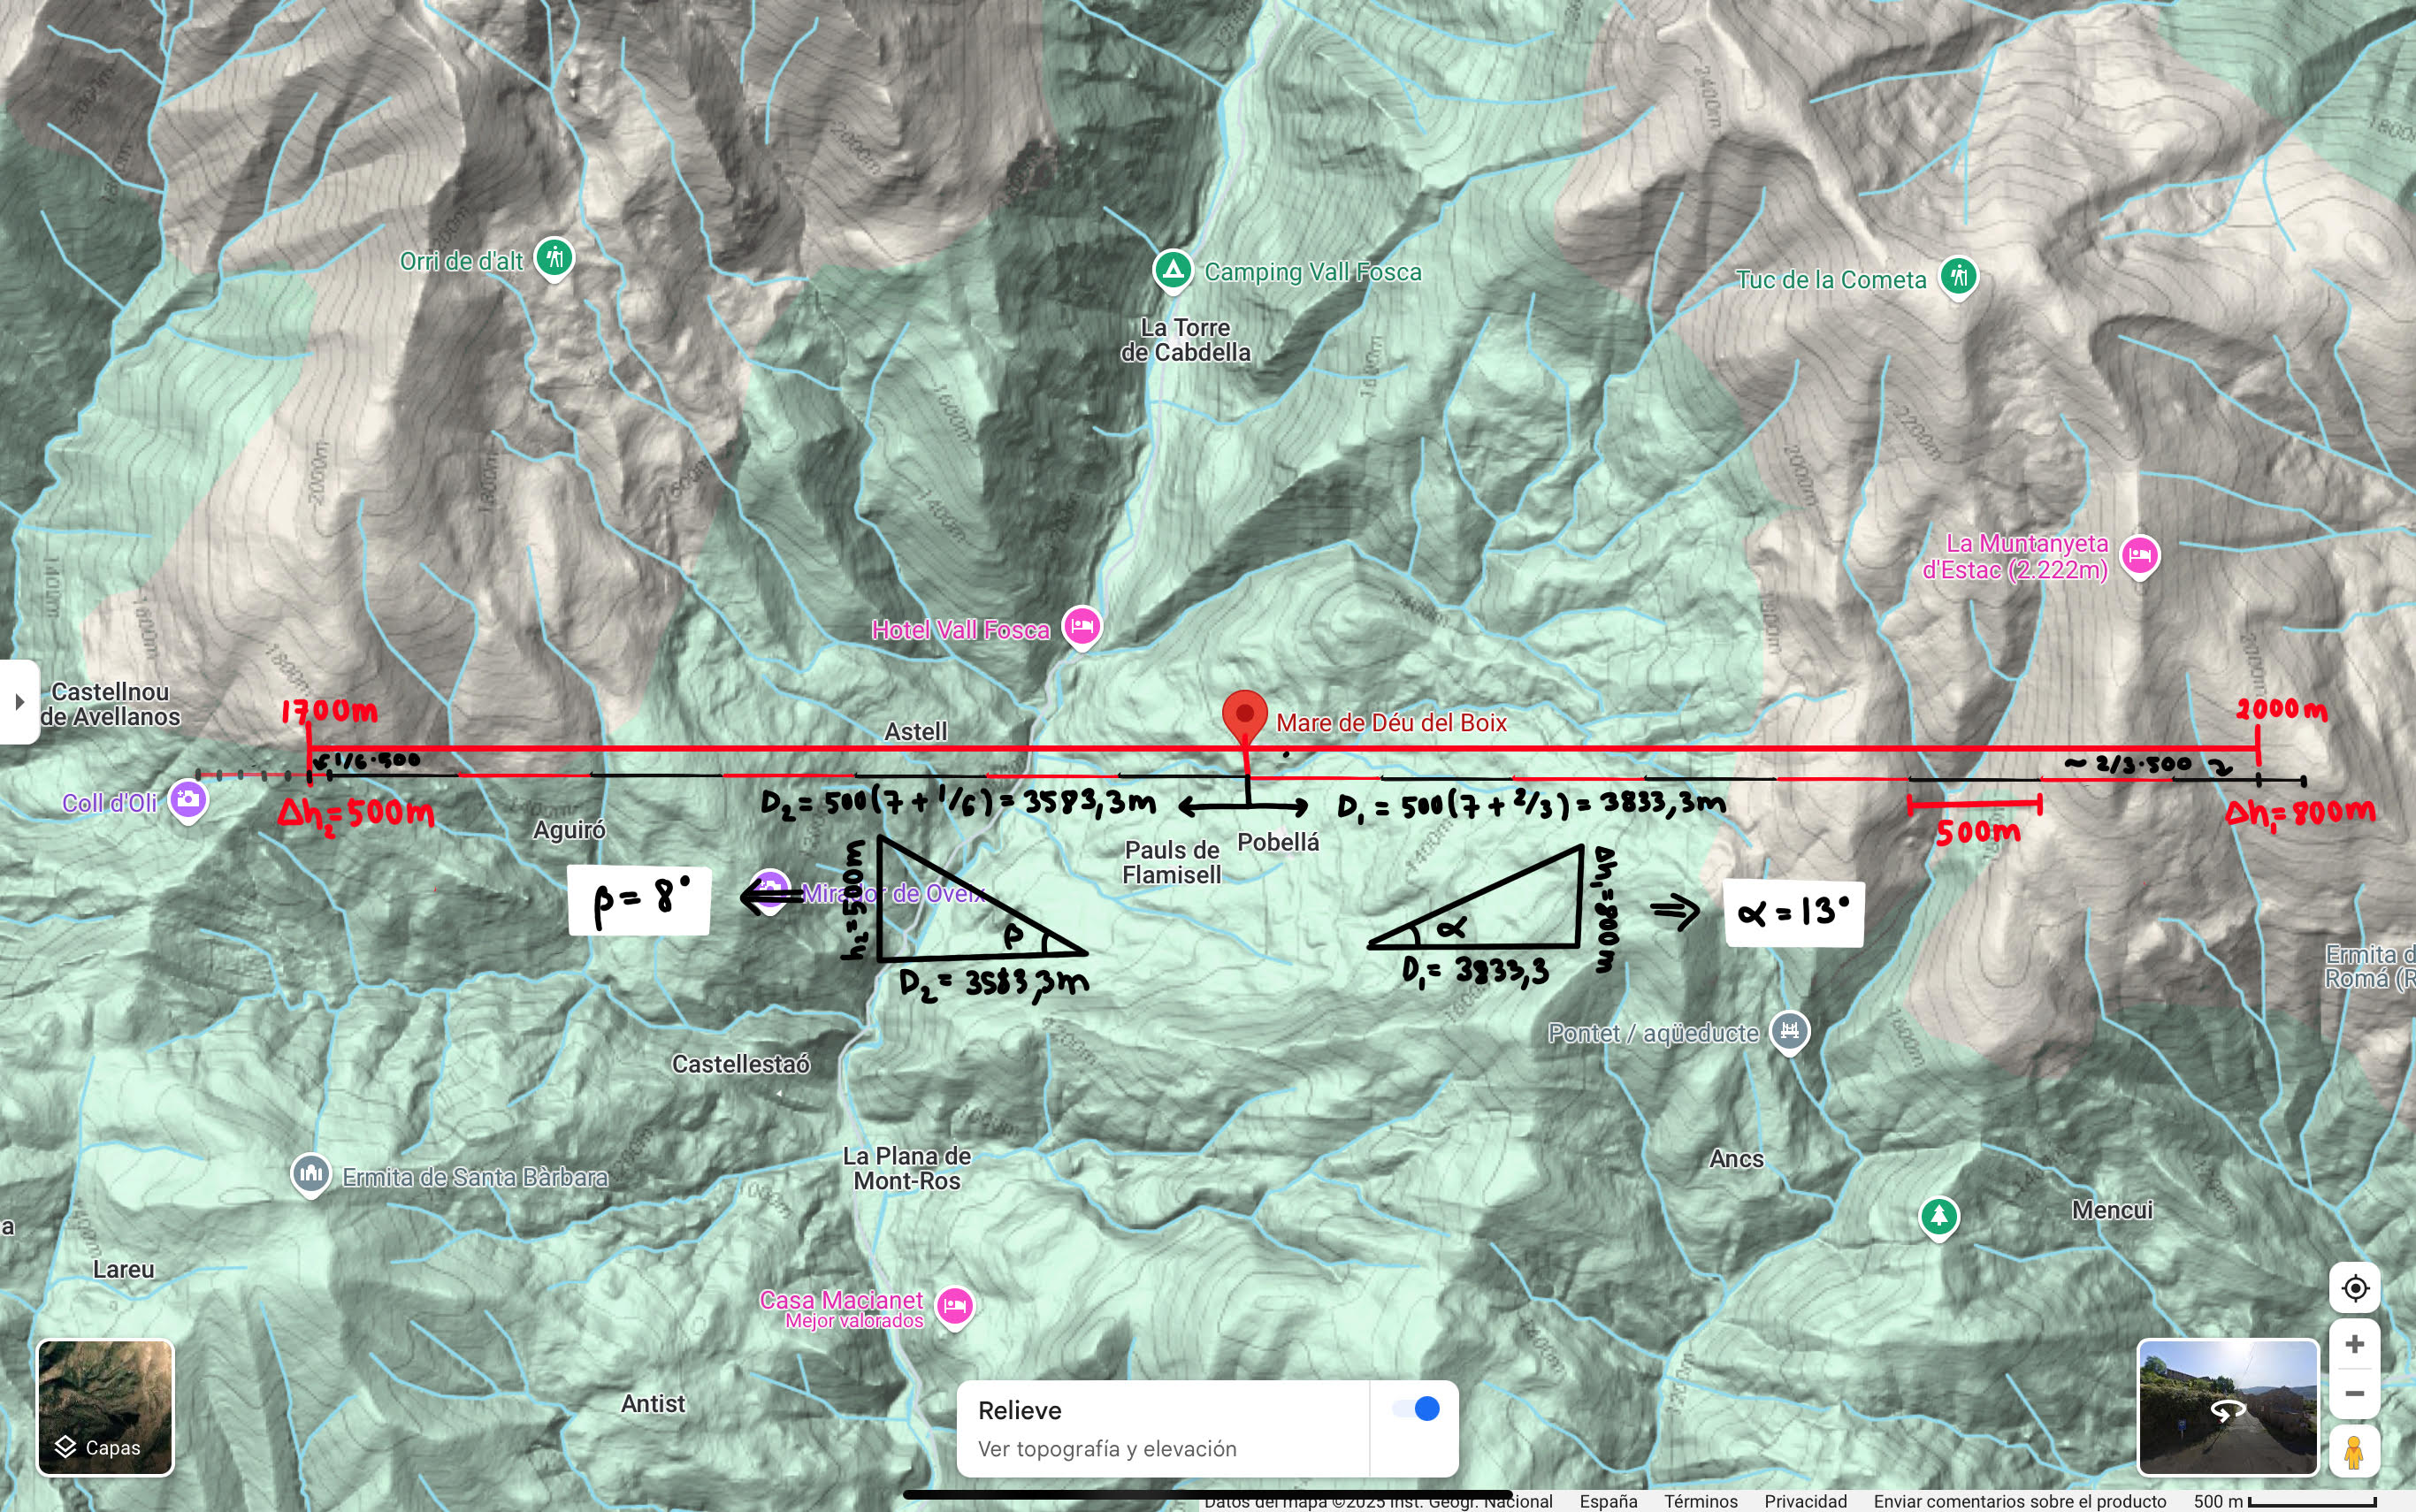
\includegraphics[width=0.7\textwidth]{MapaMuntanyes.jpg}
        \caption{Alçada relativa de les muntanyes properes a Mont-rós. Extret de \textit{Google Maps}. }
        \label{fig:alçada_muntanyes}
    \end{figure}
    \item Les precipitacions lleus no només no afecten negativament el rendiment de les plaques fotovoltaiques, sinó que també poden ser beneficioses, netejant, per exemple, la seva superfície. En aquest context, hem considerat que la principal causa de la reducció del rendiment durant les precipitacions és la formació de núvols, els quals bloquegen la radiació solar i limiten la captació d'energia. Hem considerat que (en promig)\cite{ref9}:
    \begin{itemize}
        \item Les pluges lleus no afecten el rendiment de les plaques.
        \item Les pluges moderades (4-10 mm/h) redueixen el rendiment en un 15\%.
        \item Les pluges intenses ($>$ 10 mm/h) redueixen el rendiment en un 25\%.
    \end{itemize}
    \item Pel que fa a les nevades, segons les dades històriques al poble neva, fonamentalment, entre gener i mitjans de març. Tot i que la neu pot arribar a ser altament perjudicial sobre les plaques (bloquejant completament la llum solar), la inclinació de les plaques (de 42.5 º) redueix considerablement aquest risc, així que es negligirà. A tot això cal afegir que les nevades a la zona són puntuals i de baixa intensitat, fet que facilita el desglaç i que la neu acumulada als voltants de la placa podria crear un efecte reflectant, incrementant així la captació solar.
    En cas necessari es pot instal·lar un sistema antidesglaç o una cobertura hidrofòbica, tot i que aquestes opcions consumirien part de l'energia generada. 
    Tenint en compte tots els factors comentats s'ha aplicat un factor de reducció del 20\% al rendiment durant el període de neu, com a estimació conservadora.
    \item Les plaques fotovoltaiques comencen a perdre, en general, eficiència a temperatures superiors a $T=25$ ºC, reduint-se el rendiment en un 0.3\%/ºC \cite{ref8}. A Mont-rós, les temperatures són generalment baixes, amb un clima fred a causa de la seva altitud. El problema de la temperatura només es presentaria, doncs, a l'estiu, quan les temperatures poden superar, segons els registres històrics, els 25 ºC entre les 12:00 i les 15:00 hores, arribant a màximes de 31 ºC però en períodes breus. 
    Així doncs, hem considerat que els efectes associats a la temperatura no afecten significativament el rendiment de la placa fotovoltaica.

\end{itemize}

\begin{figure}[h!]
    \centering
    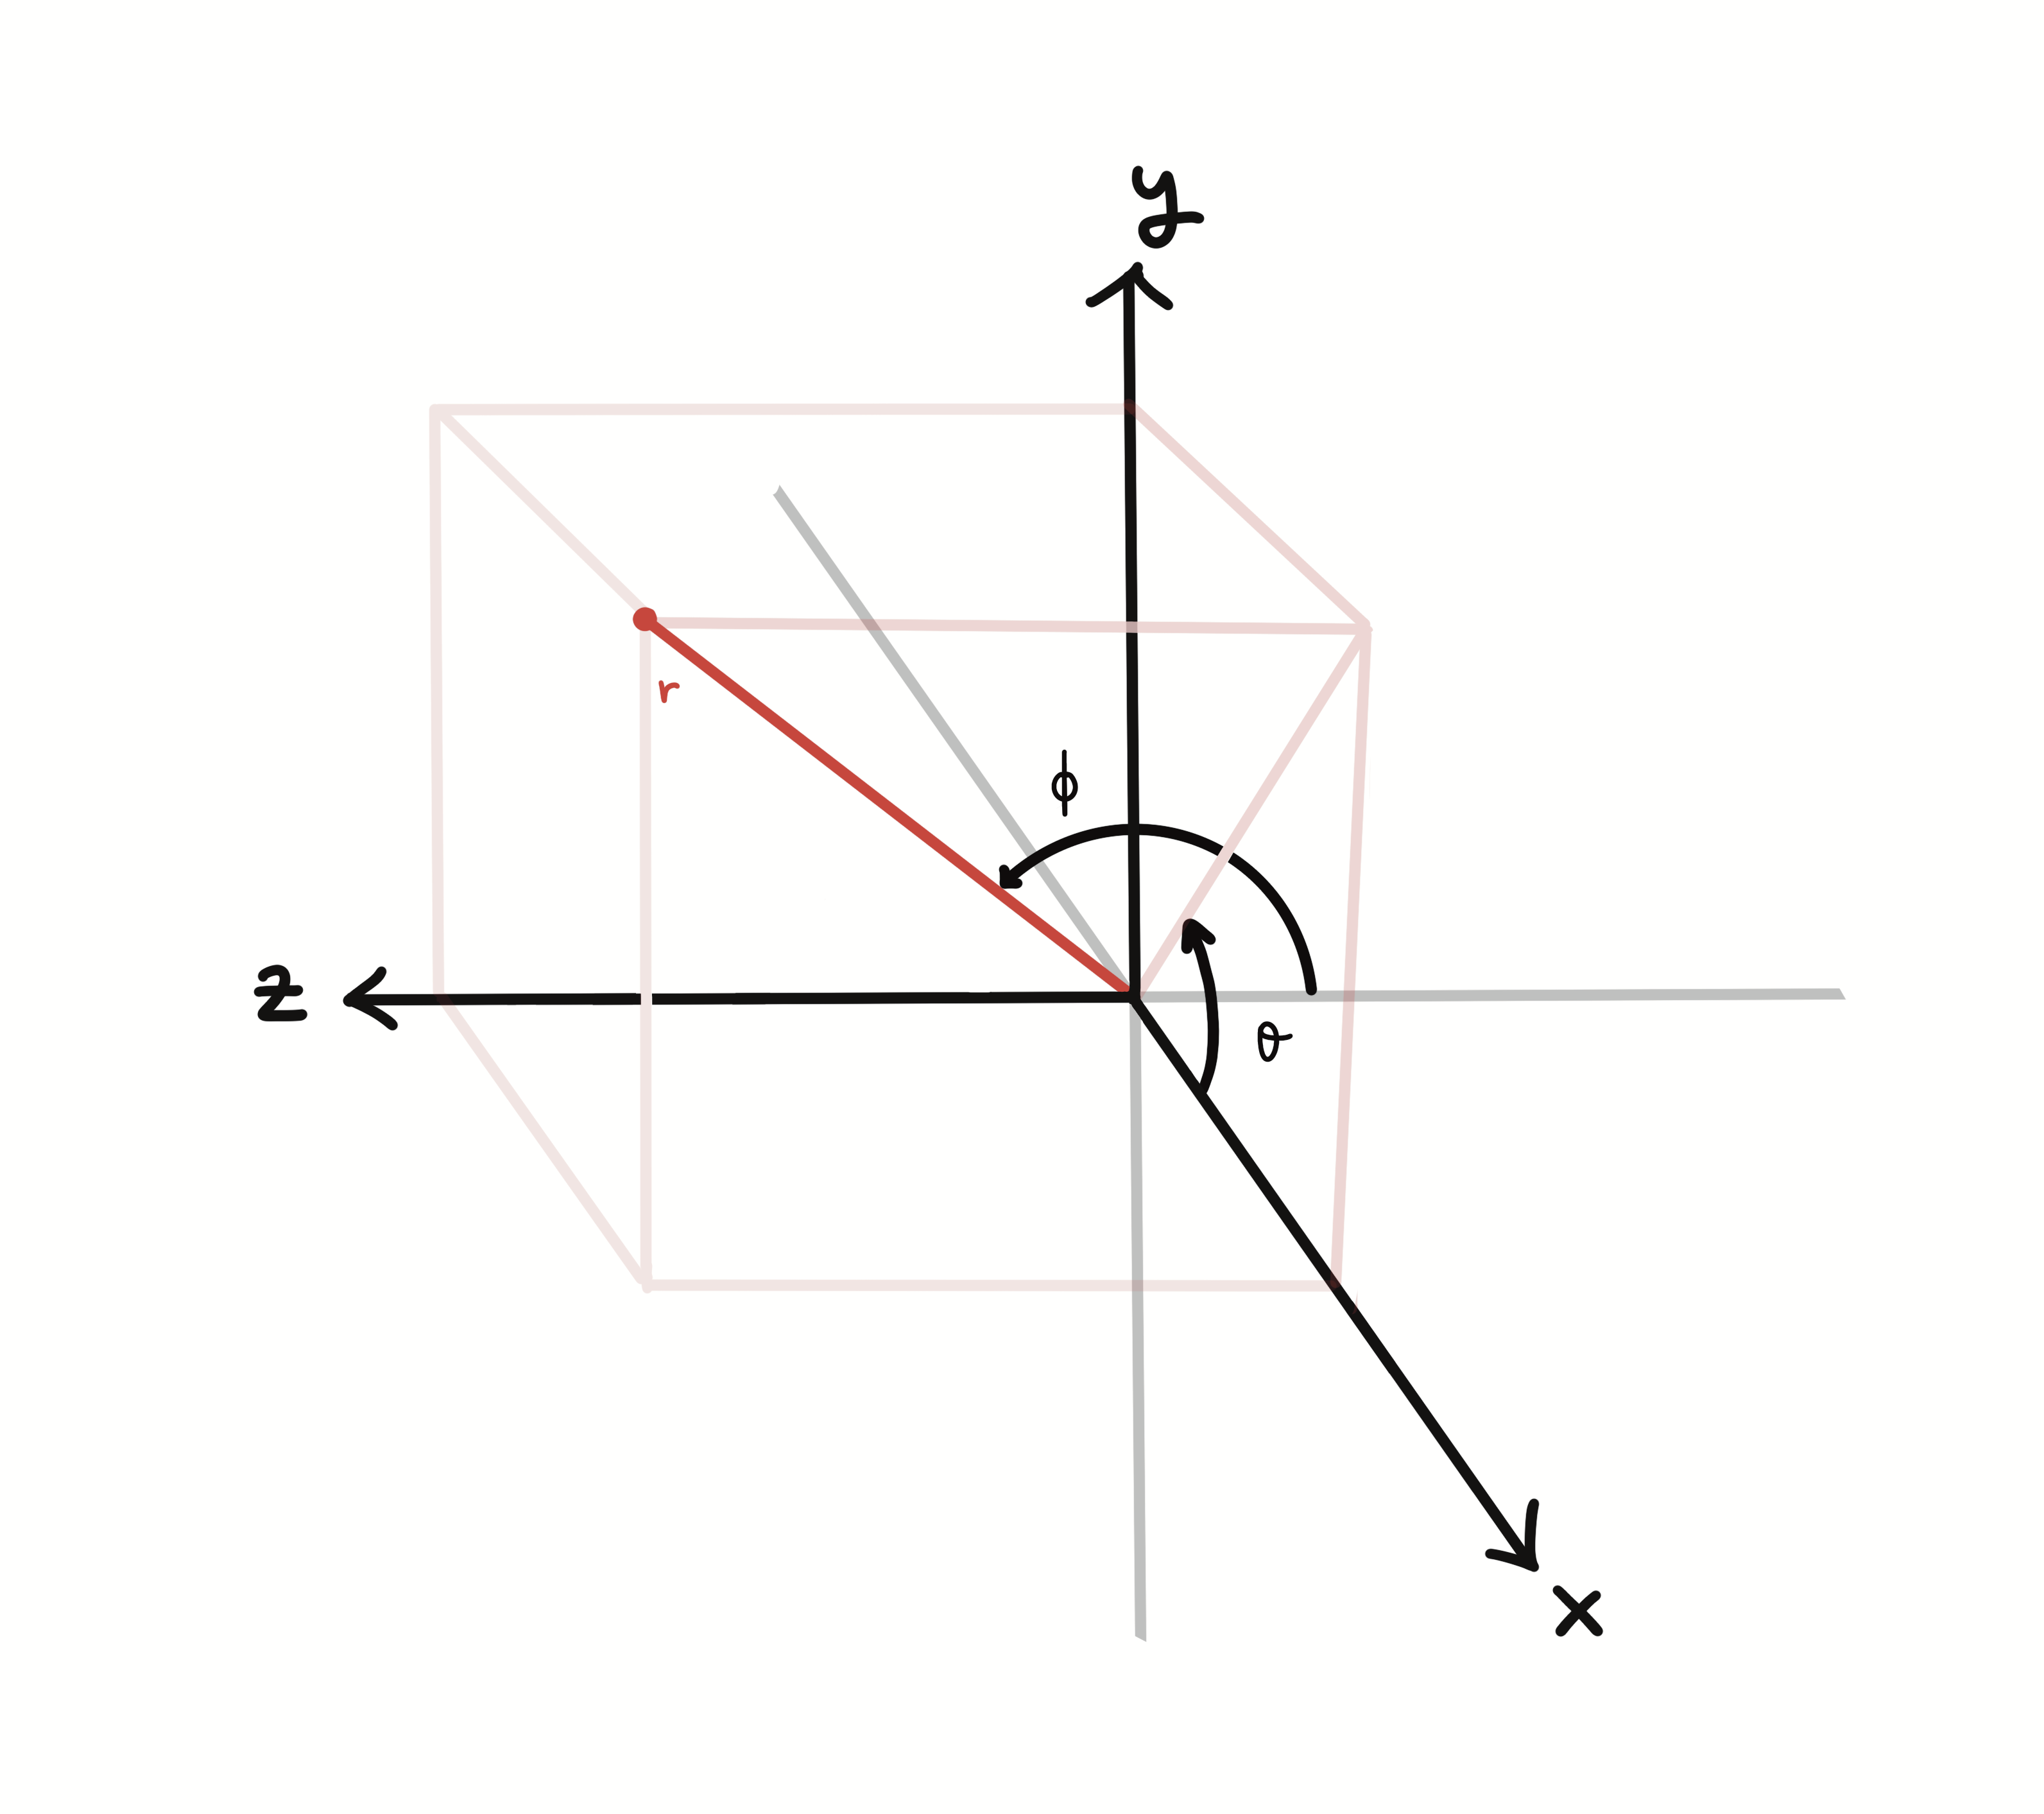
\includegraphics[width=0.5\linewidth]{../latex/Coordenades.png}
    \caption{Sistema de referència usant els angles $\phi$ i $\theta$. El pla format pels eixos $z-y$ es correspon amb la placa fotovoltaica. El vector normal a la placa té direcció $\hat{e}_x$.}
    \label{fig:sr}
\end{figure}

\subsection{Avaluació de l'error}
Per tal d'evaluar com d'exacte és el nostre model, els resultats obtinguts es compararan amb els del PVGIS \cite{ref7}. Calcularem l'error relatiu associat a l'energia subministrada per la placa fotovoltaica com:
\begin{equation}
    E_{placa} = \frac{\abs{\varepsilon_{model}-\varepsilon_{teo}}}{\varepsilon_{teo}}\cdot 100
\end{equation}
on $\varepsilon_{model}$ i $\varepsilon_{teo}$ són les energies associades al nostre model i als resultats obtinguts del PVGIS, respectivament.

\section{Resultats i discussió}

\subsection{Sistema Solar}
Després d'implementar el mètode numèric s'han trobat les òrbites (per a cada valor de $dt$) fins a $t=1$ any (terrestre) que es poden veure a les figures \ref{fig1}a, \ref{fig2}a i \ref{fig3}a. Més tard, a la figura \ref{fig4}, podem veure les òrbites per a $t=100$ anys per la discretització $dt=1$ dia amb el corresponent error.
 
A l'annex \ref{an:a} podeu trobar les gràfiques corresponents a tot el Sistema Solar (amb els cossos no descrits aquí) i un seguit d'animacions per tal de visualitzar més clarament l'evolució temporal de tots els cossos fins a un $t_{final}=15$ anys.

Els errors relatius en l'energia associats als diferents planetes es poden veure a les figures \ref{fig1}b, \ref{fig2}b i \ref{fig3}b.

\begin{figure}[h]
    \centering
    
    \begin{subfigure}[b]{0.495\linewidth}
        \centering
        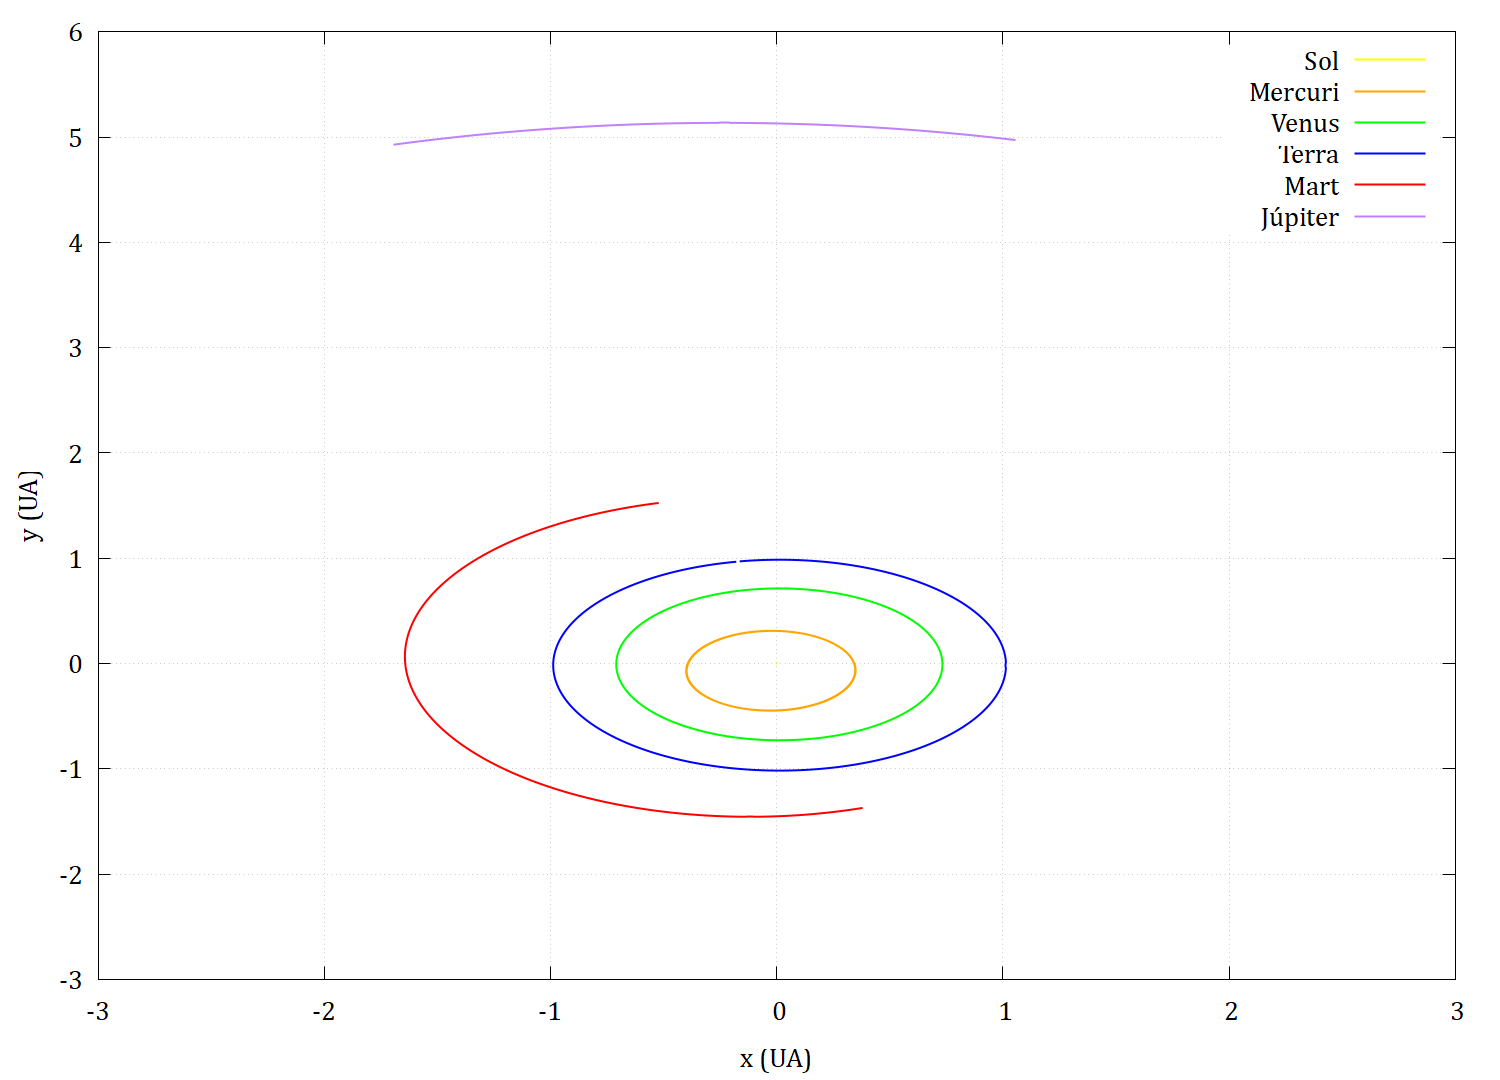
\includegraphics[width=\linewidth]{../sist_solar/orbites_euler_1_d1dia.png}
        \caption{Òrbites per $dt=1$ hora.}
    \end{subfigure}
    \hfill
    \begin{subfigure}[b]{0.495\linewidth}
        \centering
        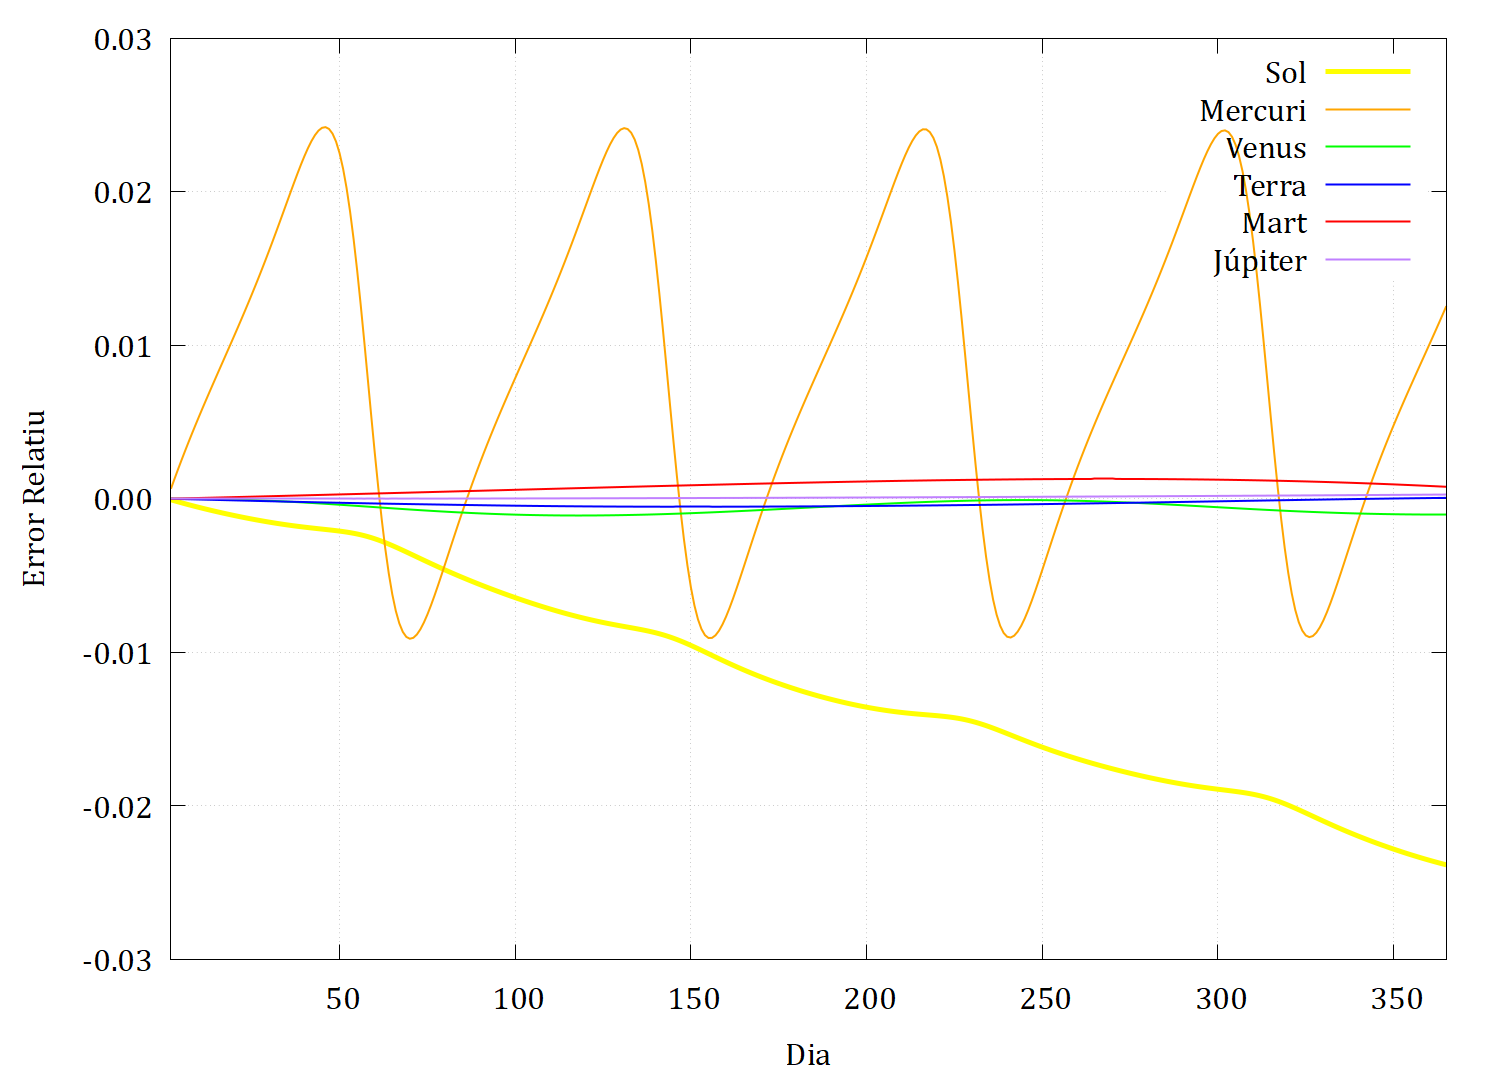
\includegraphics[width=\linewidth]{../Error/error_1_dia.png}
        \caption{Errors per $dt=1$ dia.}
    \end{subfigure}
    \caption{Òrbites del sistema solar (esquerra) i errors relatius associats a aquestes (dreta) per $dt=1$ dia fins a $t_{final}=1$ any.}
    \label{fig1}
\end{figure}

\begin{figure}[h]
    \centering
    
    \begin{subfigure}[b]{0.495\linewidth}
        \centering
        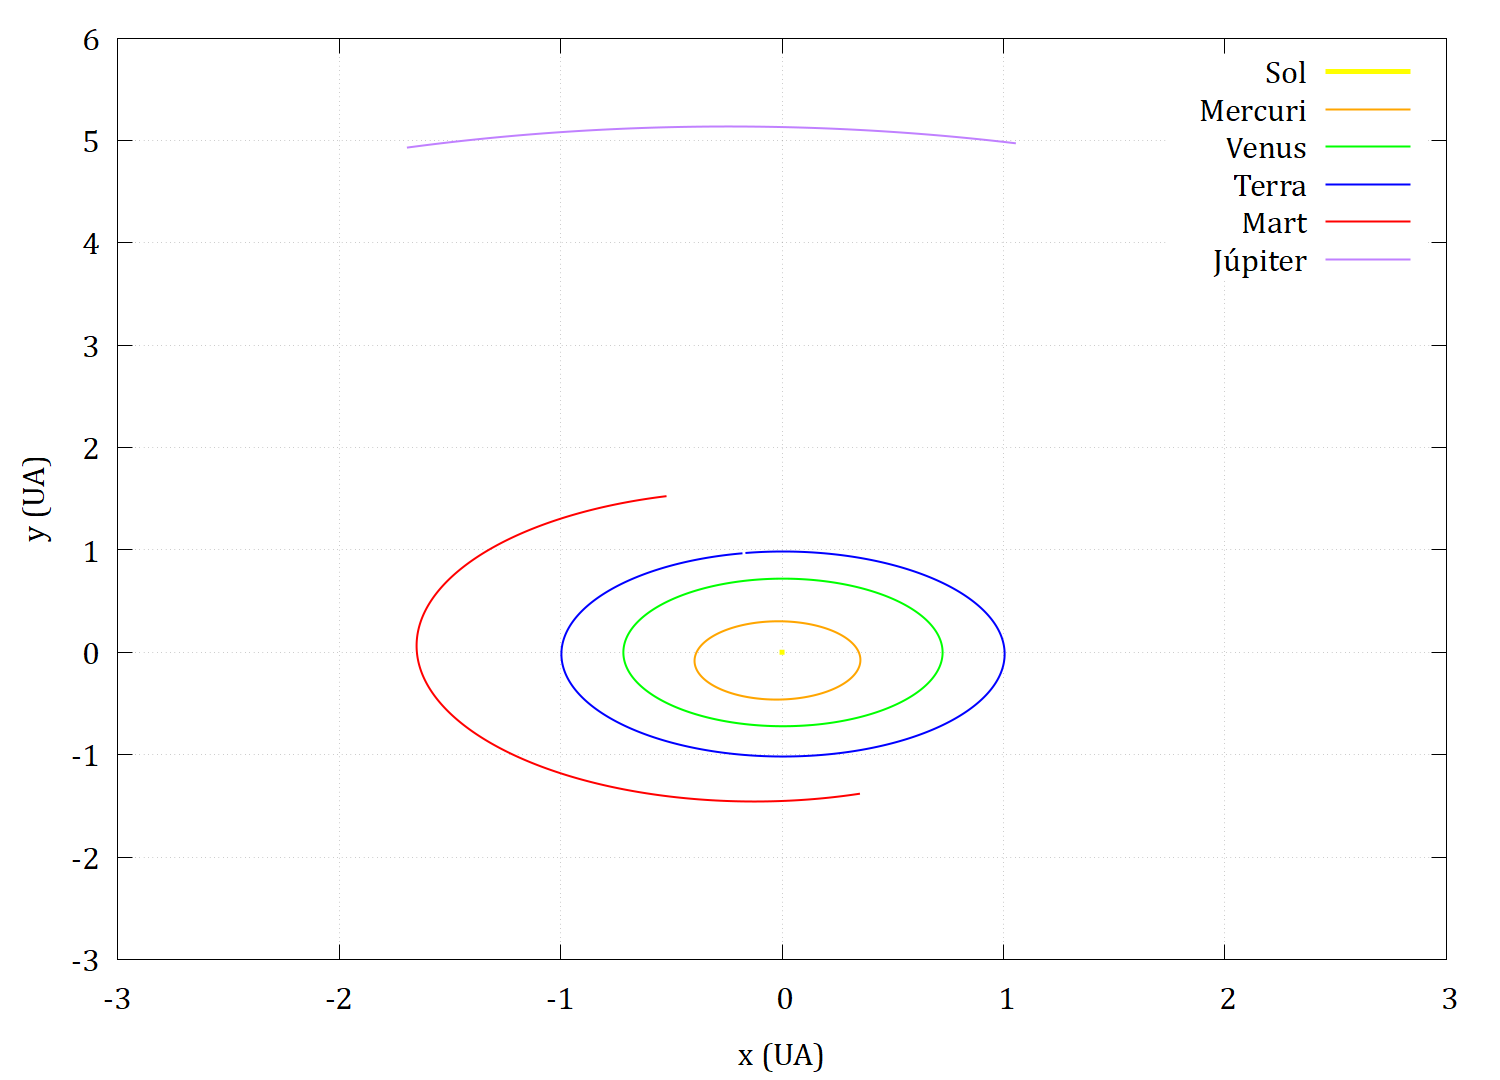
\includegraphics[width=\linewidth]{../sist_solar/orbites_euler_1_d1hora.png}
        \caption{Òrbites per $dt=1$ hora.}
    \end{subfigure}
    \hfill
    \begin{subfigure}[b]{0.495\linewidth}
        \centering
        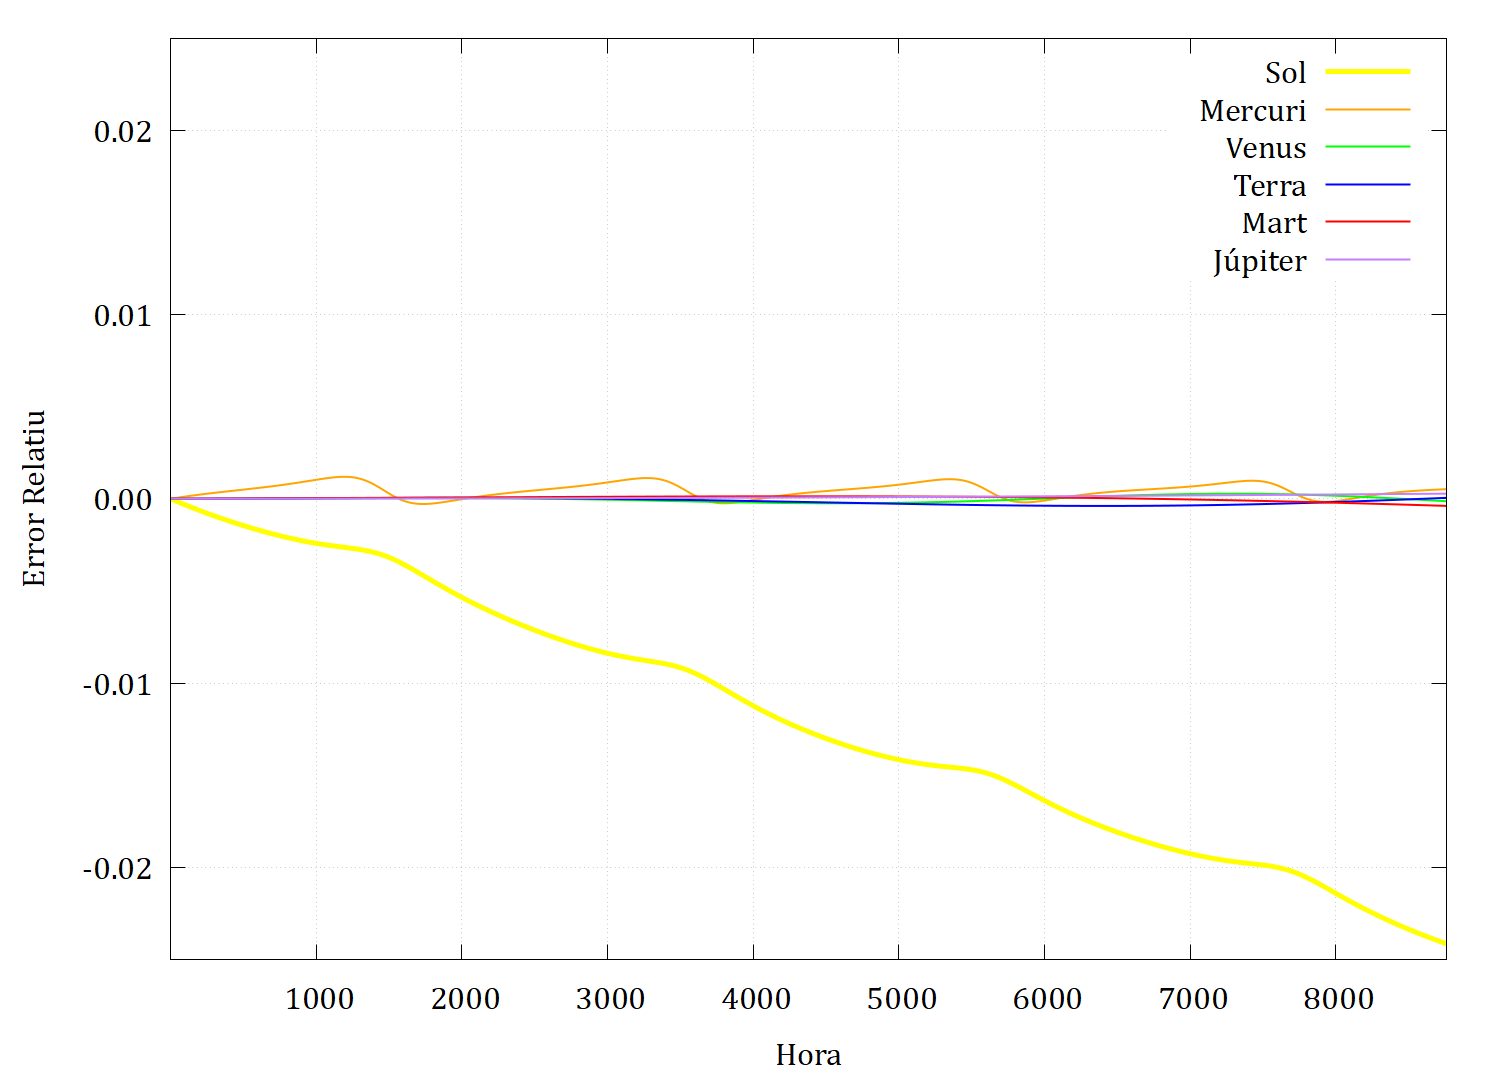
\includegraphics[width=\linewidth]{../Error/error_1_hora.png}
        \caption{Errors per $dt=1$ hora.}
    \end{subfigure}
    \caption{Òrbites del sistema solar (esquerra) i errors relatius associats a aquestes (dreta) per $dt=1$ hora fins a $t_{final}=1$ any.}
    \label{fig2}
\end{figure}

\begin{figure}[h]
    \centering
    
    \begin{subfigure}[b]{0.495\linewidth}
        \centering
        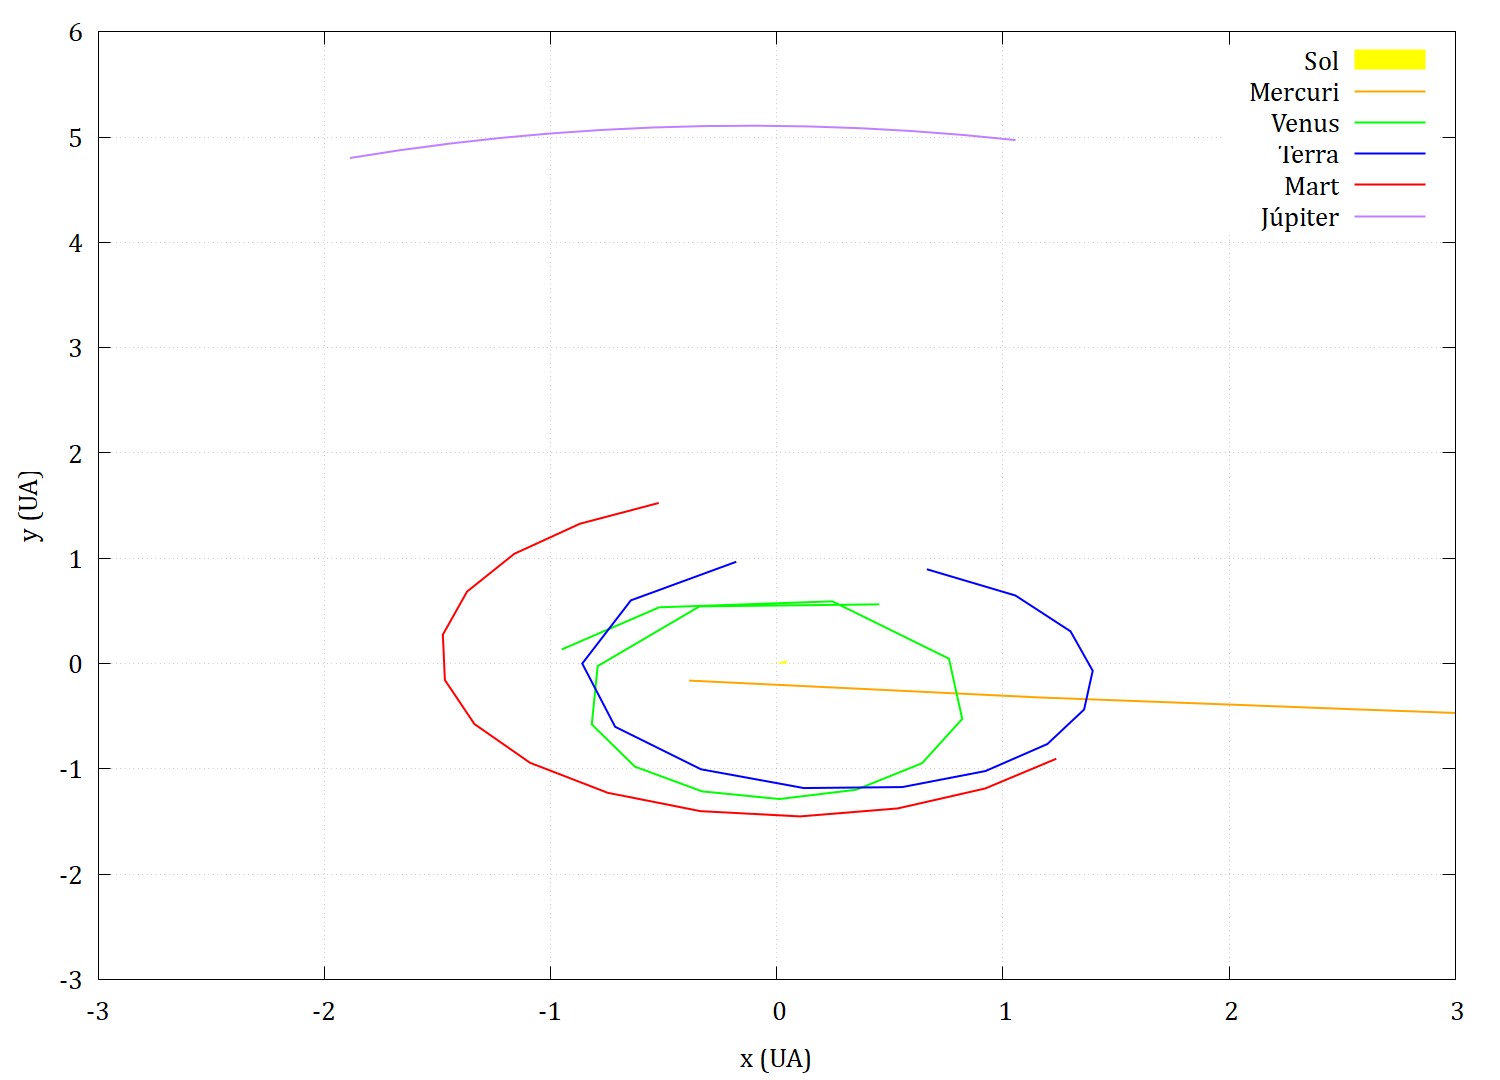
\includegraphics[width=\linewidth]{../sist_solar/orbites_euler_1_d1mes.png}
        \caption{Òrbites per $dt=1$ mes.}
    \end{subfigure}
    \hfill
    \begin{subfigure}[b]{0.495\linewidth}
        \centering
        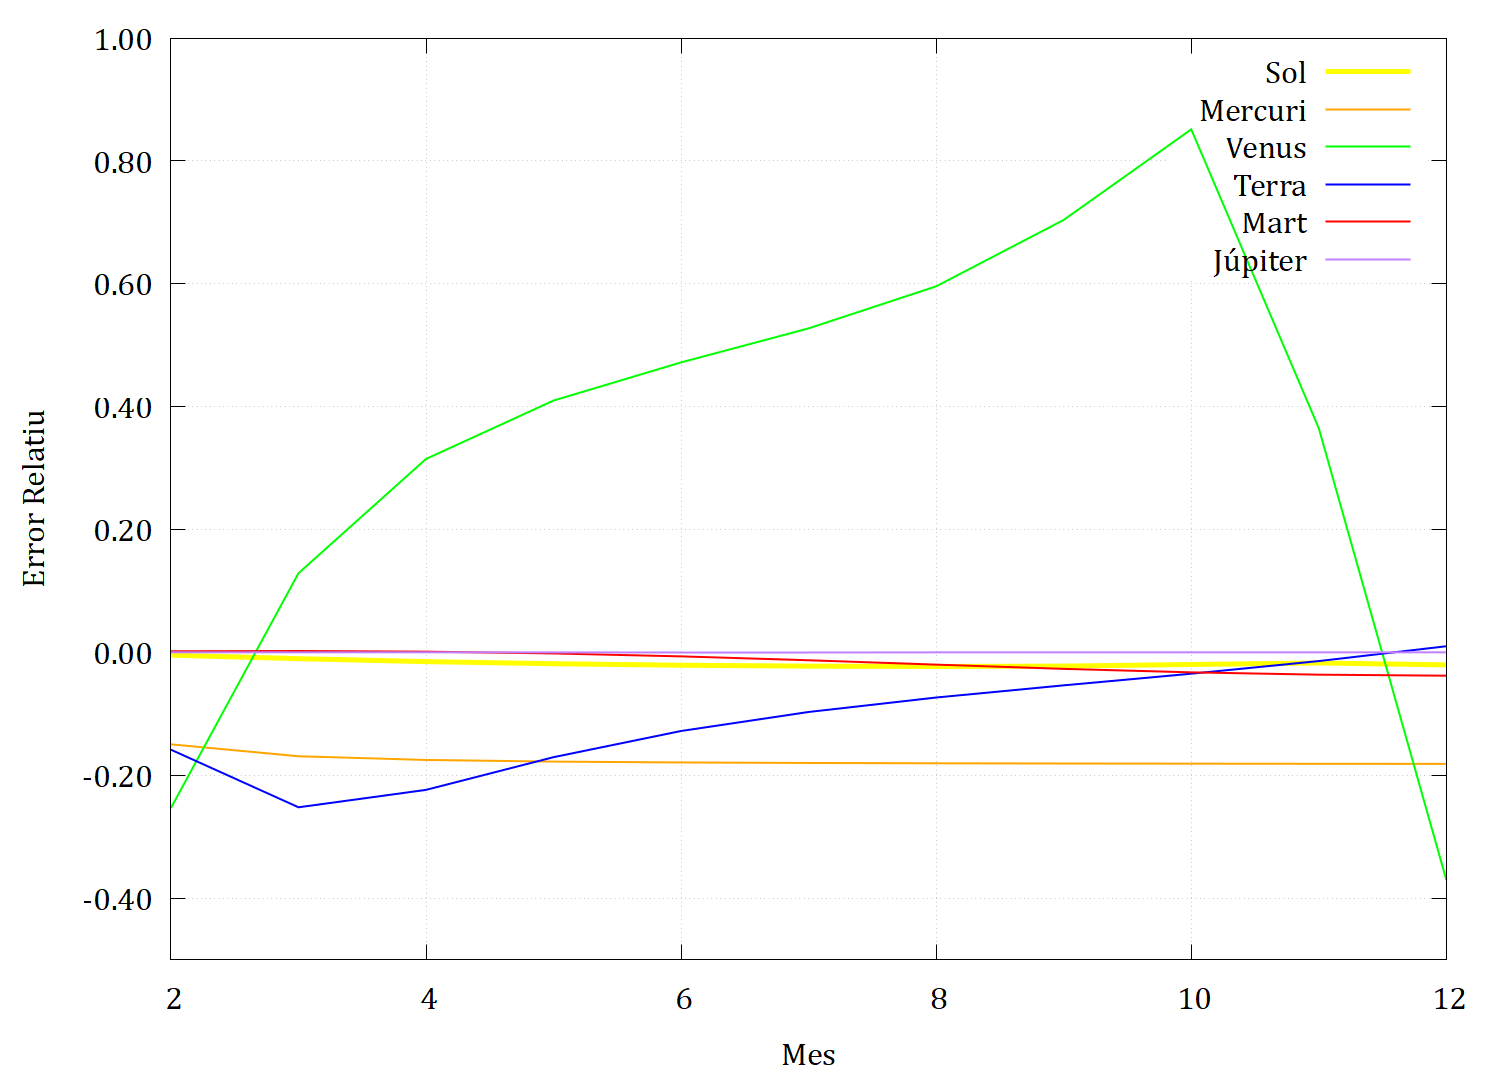
\includegraphics[width=\linewidth]{../Error/error_1_mes.png}
        \caption{Errors per $dt=1$ mes.}
    \end{subfigure}
    \caption{Òrbites del sistema solar (esquerra) i errors associats a aquestes (dreta) per $dt=1$ mes fins a $t_{final}=1$ any.}
    \label{fig3}
\end{figure}

Tal i com podem veure a la figura \ref{fig3}b, la discretització amb un major error numèric és la corresponent a $dt = 1$ mes, degut a que els grans salts en el temps fan que els errors asssociats al mètode d'Euler es disparin. En concret, podem veure com l'error associat a l'energia de Venus s'arriba a disparar fins a més d'un 80\%. La Terra i Mercuri tenen també errors relatius grans, sobretot al principi, essent aquests propers al 20\% (valor absolut). 

De fet, si ens fixem en la figura \ref{fig3}a, podem veure que Mercuri surt disparat del Sistema Solar. Que això no es vegi reflectit, aparentment, en l'error associat a l'energia de Mercuri (que es manté pràcticament constant en una desviació del 20\%) pot ser degut a què les variacions en els termes en l'energia cinètica i l'energia potencial d'aquest cos es compensen conforme l'astre s'allunya de la seva posició inicial.

Tant a la discretització de $dt = 1$ dia com a la de $dt = 1$ hora (figures \ref{fig1} i \ref{fig2}, respectivament) tenim errors associats als planetes més exteriors del sistema modelitzat similars, essent aquests lleugerament menors en el cas de la discretització per hores, a costa d'un temps de càlcul major. La principal diferència rau, però, en l'error associat a Mercuri: per a la discretització en dies presenta un error relatiu molt major al de la resta de cossos (exceptuant el Sol), assolint pics de fins a un 2.5\%; per a la discretització en hores aquest efecte es disminueix significativament.

El cas del Sol és diferent; per a les tres discretitzacions presenta una evolució de l'error associat a l'energia molt similar. En tots els casos calculats té una clara tendència a desviar-se negativament. Podem explicar això si pensem en què el Sol és, dels 6 cossos modelitzats, el que ha tenir posicions i velocitats menors, de forma que l'acumulació d'errors associats al mètode numèric pot fer que aquestes petites quantitats es vegin afectades de forma significativa.

Si fem un estudi de l'evolució del Sistema Solar fins a un $t_{final}$ major, usant $dt=1$ dia, els resultats que s'obtenen són els que es poden veure a la figura \ref{fig4}.

\begin{figure}[h!]
    \centering
    \begin{subfigure}[b]{0.48\linewidth}
        \centering
        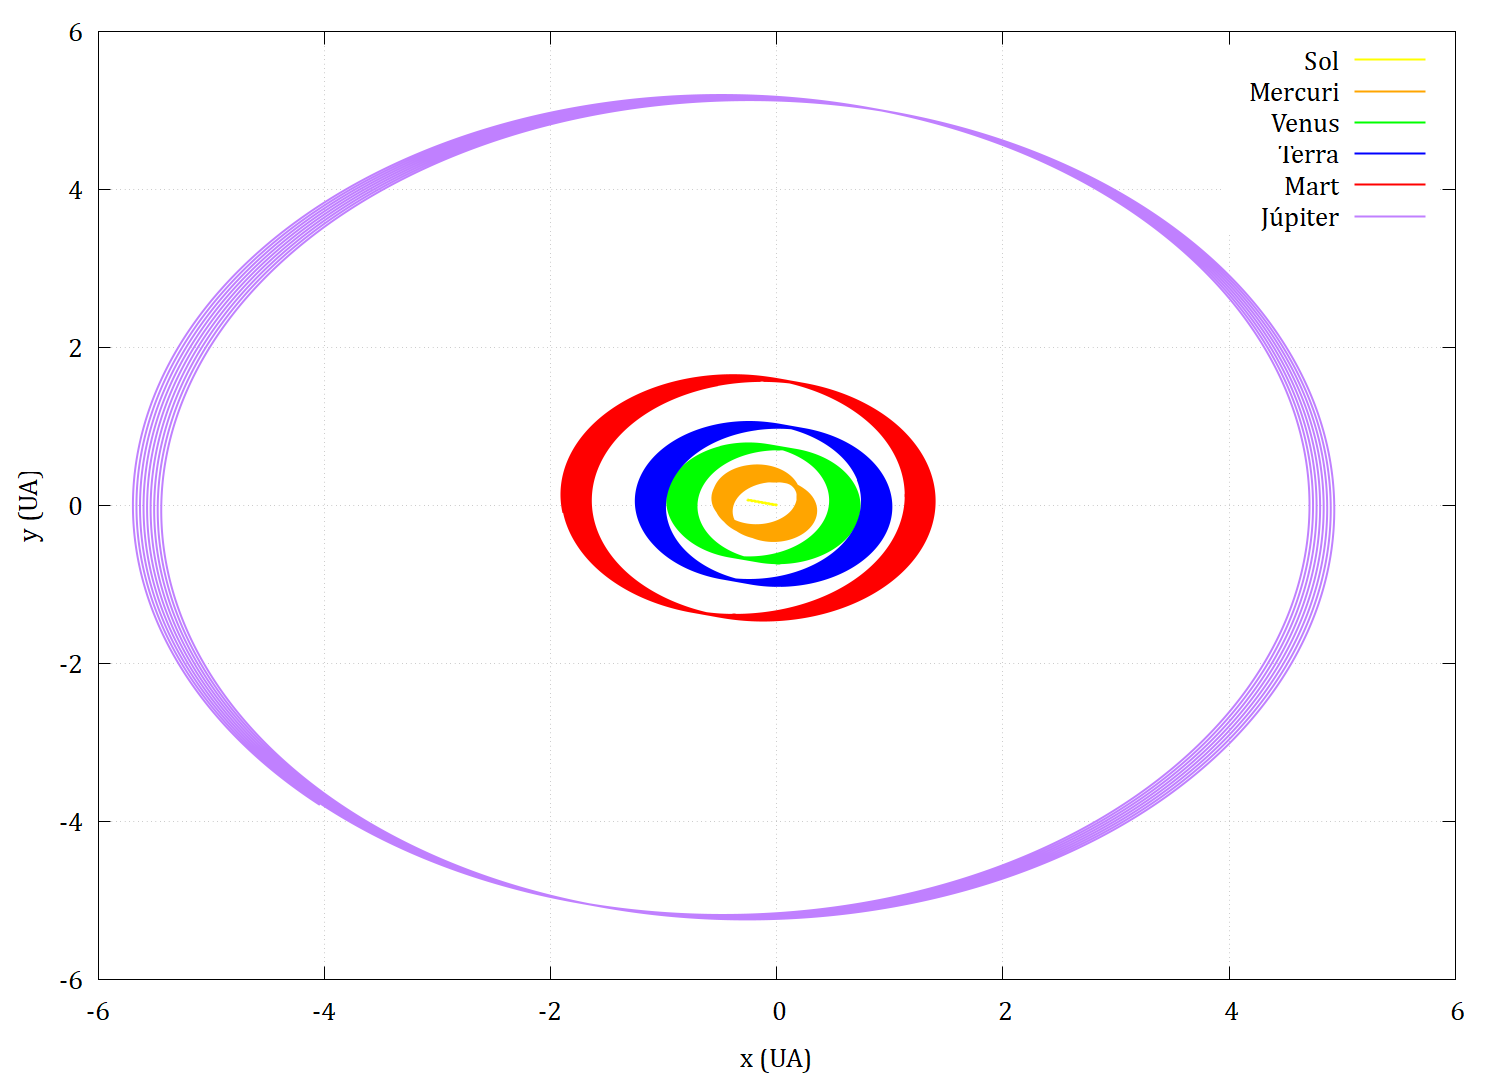
\includegraphics[width=\linewidth]{../sist_solar/orbites_euler_100_d1dia.png}
        \caption{Òrbites fins a $t_{final}=100$ anys amb $dt=1$ dia.}
    \end{subfigure}
    \hfill
    \begin{subfigure}[b]{0.48\linewidth}
        \centering
        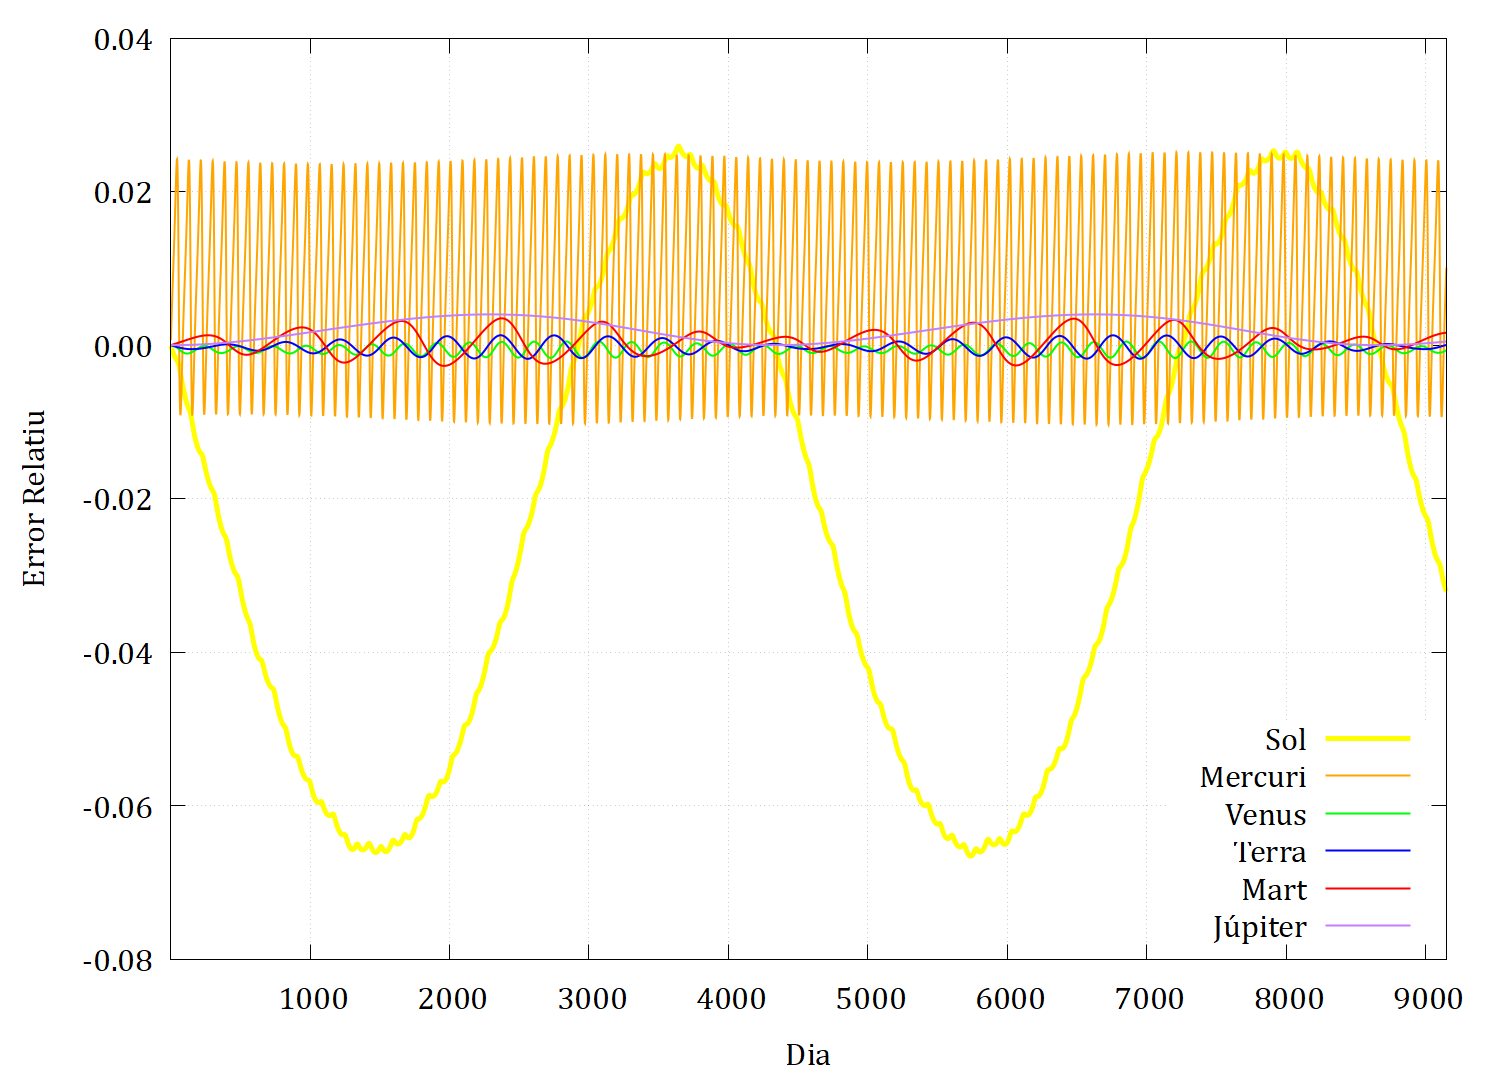
\includegraphics[width=\linewidth]{../Error/error_100_dia.png}
        \caption{Errors fins a $t_{final}=25$ anys per $dt=1$ dia.}
    \end{subfigure}
    \caption{Estudi de l'evolució del Sistema Solar a $t_{final}$ major.}
    \label{fig4}
\end{figure}

Ara es posa de manifest el caràcter oscil·latori de l'error relatiu per tots els cossos del Sistema Solar. Podem veure com l'error màxim obtingut és proper al 6.5\% (valor absolut) en el cas del Sol, pels motius ja comentats abans\footnote{Per motius de qualitat, la gràfica associada a l'error per $t_{final}=100$ anys arriba només fins al 25 anys. Podeu trobar més informació a l'enllaç de l'annex \ref{an:a}.}. La resta de planetes, exceptuant el cas de Mercuri, no arriben en cap cas a errors superiors al 1\%.

\subsection{Moviment del Sol sobre Mont-rós}
A la figura \ref{fig:solstici} s'ha representat el moviment del Sol des de Mont-rós el dia del solstici d'estiu que, pel present any 2025, és el dia 21 de juny.

Com es pot observar a la figura \ref{fig:mesos}, el moviment del Sol varia en funció de l'època de l'any que vulguem considerar. Aquesta gràfica posa també de manifest que el dia 21 de juny es correspon, efectivament, amb el solstici d'estiu, ja que és el dia que el Sol té una trajectòria més llarga, que es tradueix en hores màximes de llum. Per contra, el 21 de desembre és el solstici d'hivern, és a dir, és el dia amb un període diürn més curt.

\begin{figure}[h!]
    \centering
    \begin{minipage}{0.48\linewidth} 
        \centering
        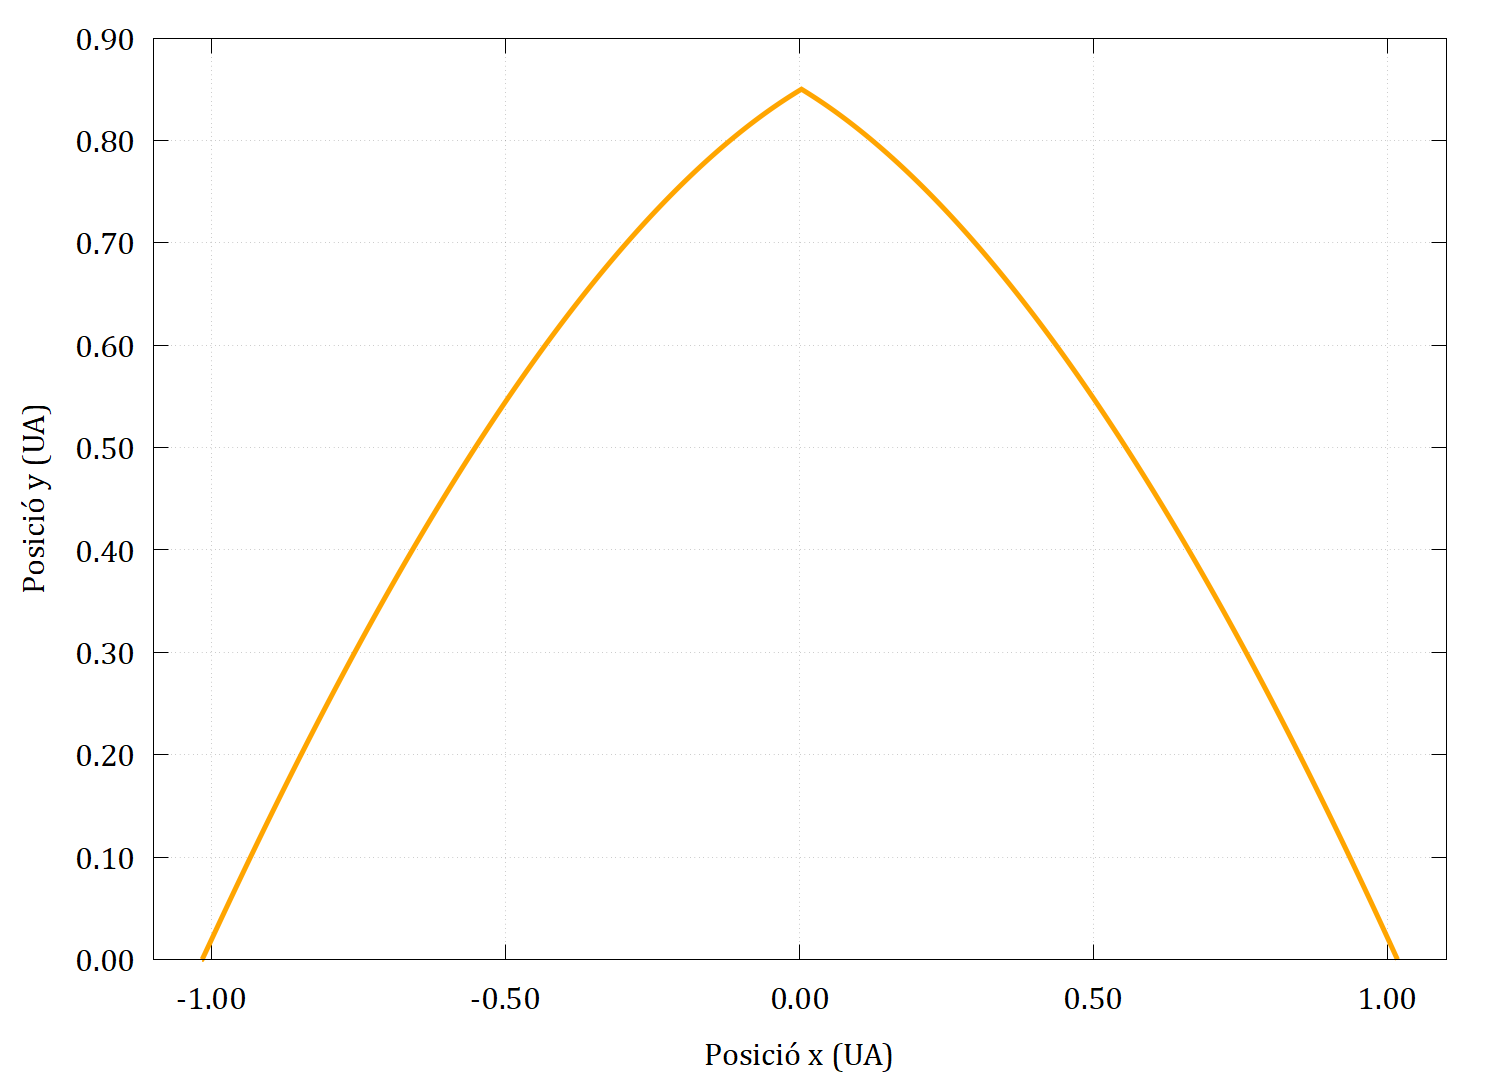
\includegraphics[width=\linewidth]{mov_sol_solstici.png}
        \caption{Moviment del Sol observat des de Mont-rós al solstici d'estiu (21 de juny del 2025).}
        \label{fig:solstici}
    \end{minipage}\hfill 
    \begin{minipage}{0.48\linewidth} 
        \centering
        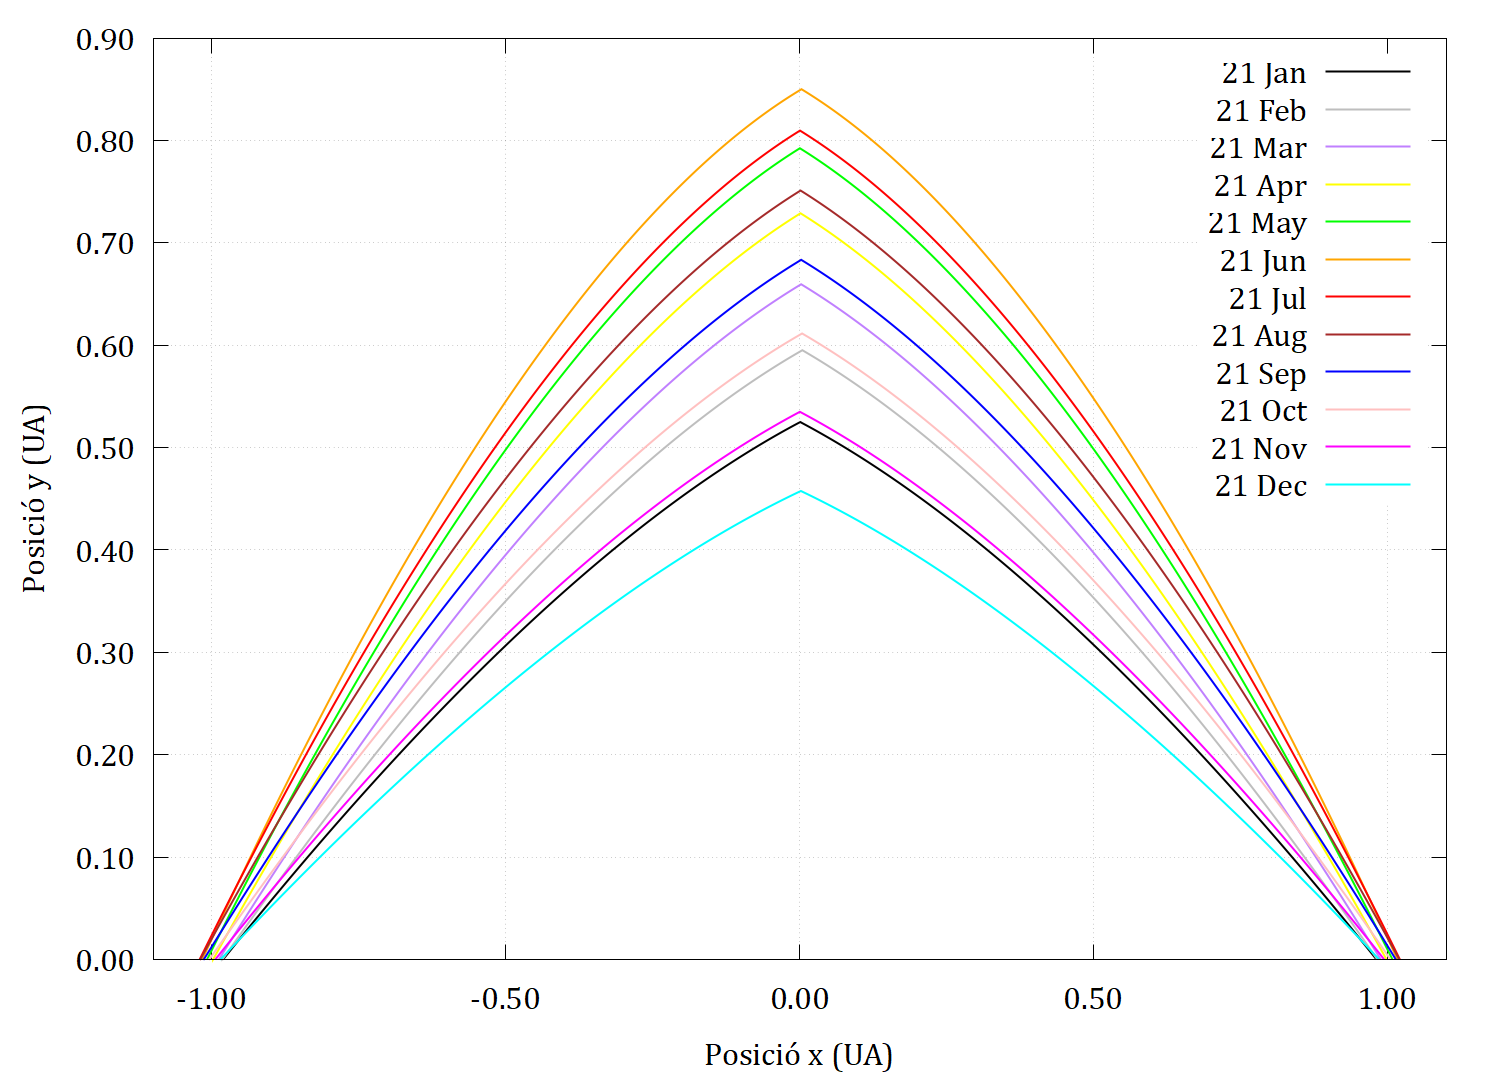
\includegraphics[width=\linewidth]{mov_sol_mesos.png}
        \caption{Moviment del Sol observat des de Mont-rós pels dies 21 de cada mes del present any 2025.}
        \label{fig:mesos}
    \end{minipage}
\end{figure}

\textbf{COMENTAR ALGUNA COSA DE COM ES MOU?}


\subsection{Energia subministrada per la placa solar}
A les figures \ref{fig:figura1} i \ref{fig:figura2} es poden observar els histogrames corresponents a l'energia elèctrica generada cada mes al llarg d'un any de la nostra placa i la obtinguda a segons el model del PVGIS. 

\begin{figure}[!ht]
    \centering
    \begin{minipage}{0.48\linewidth} 
        \centering
        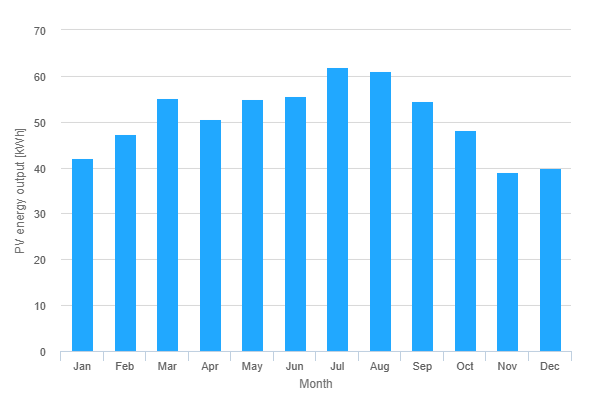
\includegraphics[width=\linewidth]{Histograma_PVGIS.png}
        \caption{Histograma de l'energia generada durant un any extreta de PVGIS}
        \label{fig:figura1}
    \end{minipage}\hfill 
    \begin{minipage}{0.48\linewidth} 
        \centering
        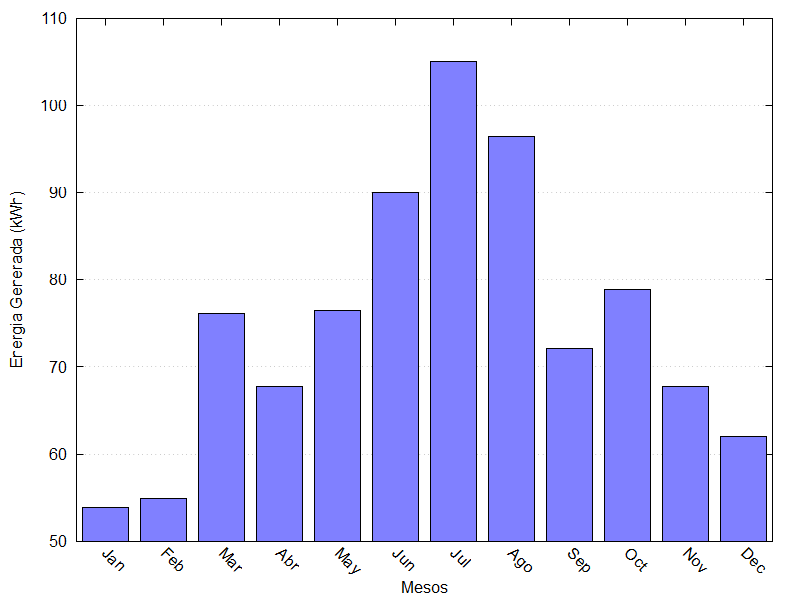
\includegraphics[width=\linewidth]{../Mov_sol/histograma.png}
        \caption{Histograma de l'energia generada durant un any del nostre model}
        \label{fig:figura2}
    \end{minipage}
\end{figure}

\begin{table}[h!]
    \centering
    \renewcommand{\arraystretch}{1.5}  % Aumenta el espacio entre filas
    \caption{Comparativa de l'energia generada (kWh) pel nostre model i el PVGIS més l'error relatiu.}
    \begin{tabular}{l*{12}{c}} 
        \hline
        \textbf{ } & \textbf{Jan} & \textbf{Feb} & \textbf{Mar} & \textbf{Abr} & \textbf{May} & \textbf{Jun} & \textbf{Jul} & \textbf{Ago} & \textbf{Sep} & \textbf{Oct} & \textbf{Nov} & \textbf{Dec} \\
        \hline
        \textbf{Model} & 54.89 & 58.01 & 77.54 & 69.18 & 78.38 & 92.25 & 106.60 & 97.40 & 73.63 & 80.01 & 68.68 & 63.00 \\
        \textbf{PVGIS} & 42.05 & 47.35 & 55.13 & 50.56 & 54.98 & 55.54 & 62.04 & 61.03 & 54.57 & 48.27 & 38.93 & 39.81 \\
        \textbf{Error (\%)} & 30.54 & 22.51 & 40.65 & 36.83 & 42.56 & 66.10 & 71.82 & 59.59 & 34.93 & 65.76 & 76.42 & 58.25 \\
        \hline
    \end{tabular}
\end{table}


Es poden observar diferències significatives en els histogrames entre els valors obtinguts pel nostre model i els valors de referència del PVGIS. Tot i això, aquestes diferències segueixen la tendència general dels valors, amb una producció d'energia més baixa durant els mesos d'hivern i una producció més elevada durant els mesos d'estiu, com era d'esperar.

\section{Conclusions}

La motivació principal d'aquesta pràctica era el càlcul de l'energia generada per una placa solar de superfície igual a 2 m$^2$ situada a Mont-rós. Per arribar a trobar aquests resultats s'ha efectuat prèviament una simulació quasi completa del Sistema Solar sota les condicions esmentades, amb el pretext de calcular quines eren les distàncies Terra-Sol en tot moment. D'això últim podem concloure que, a la vista dels resultats, tot i les limitacions ja explicades del mètode d'Euler, les òrbites resultants obtingudes són força bones, en especial si considerem la discretització $dt=1$ dia que, tot i presentar un error bastant major en el cas de Mercuri, no afecta de forma apreciable als resultats en les òrbites de la Terra, que són, al final del dia, les que ens interessen per fer la modelització de la placa solar. A tot això cal sumar-li el fet que la discretització per dies té un temps de càlcul associat molt menor si el comparem amb el de la discretització de $dt=1$ hora, cosa que justifica encara més la nostra elecció.


Els resultats obtinguts per l'energia generada són prou satisfactoris, ja que, tot i que el nostre model es basa en aproximacions i no és completament precís, proporciona valors raonables i coherents amb les expectatives. Això demostra que el model, tot i la seva simplicitat, és útil per obtenir una estimació acceptable dels valors de producció d'energia.


\textbf{(conclusions moviment sol sobre terra)}
\\
\\
\textbf{(conclusions globals)}

\newpage
\begin{thebibliography}{99}
    \bibitem{ref1}
    Escartín, J.M. i Navau, C. \textit{Mètodes Numèrics II}. Apunts de l'Assignatura (veure CV).

    \bibitem{ref2}
    Aguilar, L. \textit{Modelizando el Sistema Solar}. Consultat el: 11/12/2024. \url{https://www.astrosen.unam.mx/~aguilar/MySite/Teaching_files/BasicEqns-1.pdf}.

    \bibitem{ref3}
    \textit{Horizon Ephemeris}, NASA. Web de consulta de les posicions de tots els astres del sistema solar. Consultat el: 23/12/2024. \url{https://ssd.jpl.nasa.gov/horizons/}.

    \bibitem{ref4}
    Universidad de Granada. \textit{El Sistema Solar y las Galaxias. Una Introducción a la Dinámica Molecular}. Consultat el: 11/12/2024. \url{https://ergodic.ugr.es/cphys/LECCIONES/ssolar/planetas-SLIDES.pdf}.

    \bibitem{ref5}
    \textit{MeteoGram}. Web per a consultar els horaris de les sortides i postes del Sol a tot el planeta. Consultat el: 05/01/2025. \url{https://meteogram.es/sol/espana/vielha/}.

    \bibitem{ref6}
    \textit{NASA Power}, NASA. Web per consultar la metereología de qualsevol lloc del món. Consultat el 07/01/2025. \url{https://power.larc.nasa.gov/data-access-viewer/}.

    \bibitem{ref7}
    \textit{Photovoltaic Geographical Information System (PVGIS)}. Web oficial de la Comissió Europea per a consultar informació sobre la radiació solar i sobre el rendiment i l'energia generada per plaques fotovoltaiques a qualsevol lloc del planeta (a excepció del Pol Nord i el Pol Sud). Consultat el 08/01/2025. \url{https://joint-research-centre.ec.europa.eu/photovoltaic-geographical-information-system-pvgis_en}.

    \bibitem{ref8}
    \textit{¿Cómo la temperatura afecta a las placas solares?}. Consultat el 06/01/2025. \url{https://www.sfe-solar.com/noticias/articulos/efecto-de-la-temperatura-en-los-paneles-solares/}

    \bibitem{ref9}
    \textit{¿Influye la lluvia en el rendimiento de los paneles solares?}. Consultat el 06/01/2025. \url{https://energiaycalorextremadura.es/fotovoltaica/influye-la-lluvia-en-el-rendimiento-de-los-paneles-solares/}
\end{thebibliography}

\newpage
\appendix
{\Huge{\textbf{Annexos}}}
\section{Repositori de \textit{GitHub}}
\label{an:a}
Podeu trobar els codis usats en \textit{Fortran}, les representacions de les gràfiques usant \textit{Gnuplot}, animacions de les simulacions del sistema solar i més al següent repositori (públic) de \textit{GitHub}: \url{https://github.com/elitus7/PSimulacio_MN2}.

\section{Simulació del Sistema Solar amb més cossos}
\label{an:b}
A mode d'extra, afegim en aquest annex els resultats de la simulació del Sistema Solar considerant també Saturn, Urà i Neptú (més enllà dels cossos del model del text principal) mantenint, però, la condició que el moviment es dóna en un únic pla. A la figura \ref{fig:an1} podeu veure les òrbites obtingudes usant una discretització de $dt=1$ dia, que com hem vist és la millor pel que fa a temps de càlcul i exactitud, i un $t_{final}=150$ anys.

\begin{figure}[h]
    \centering
    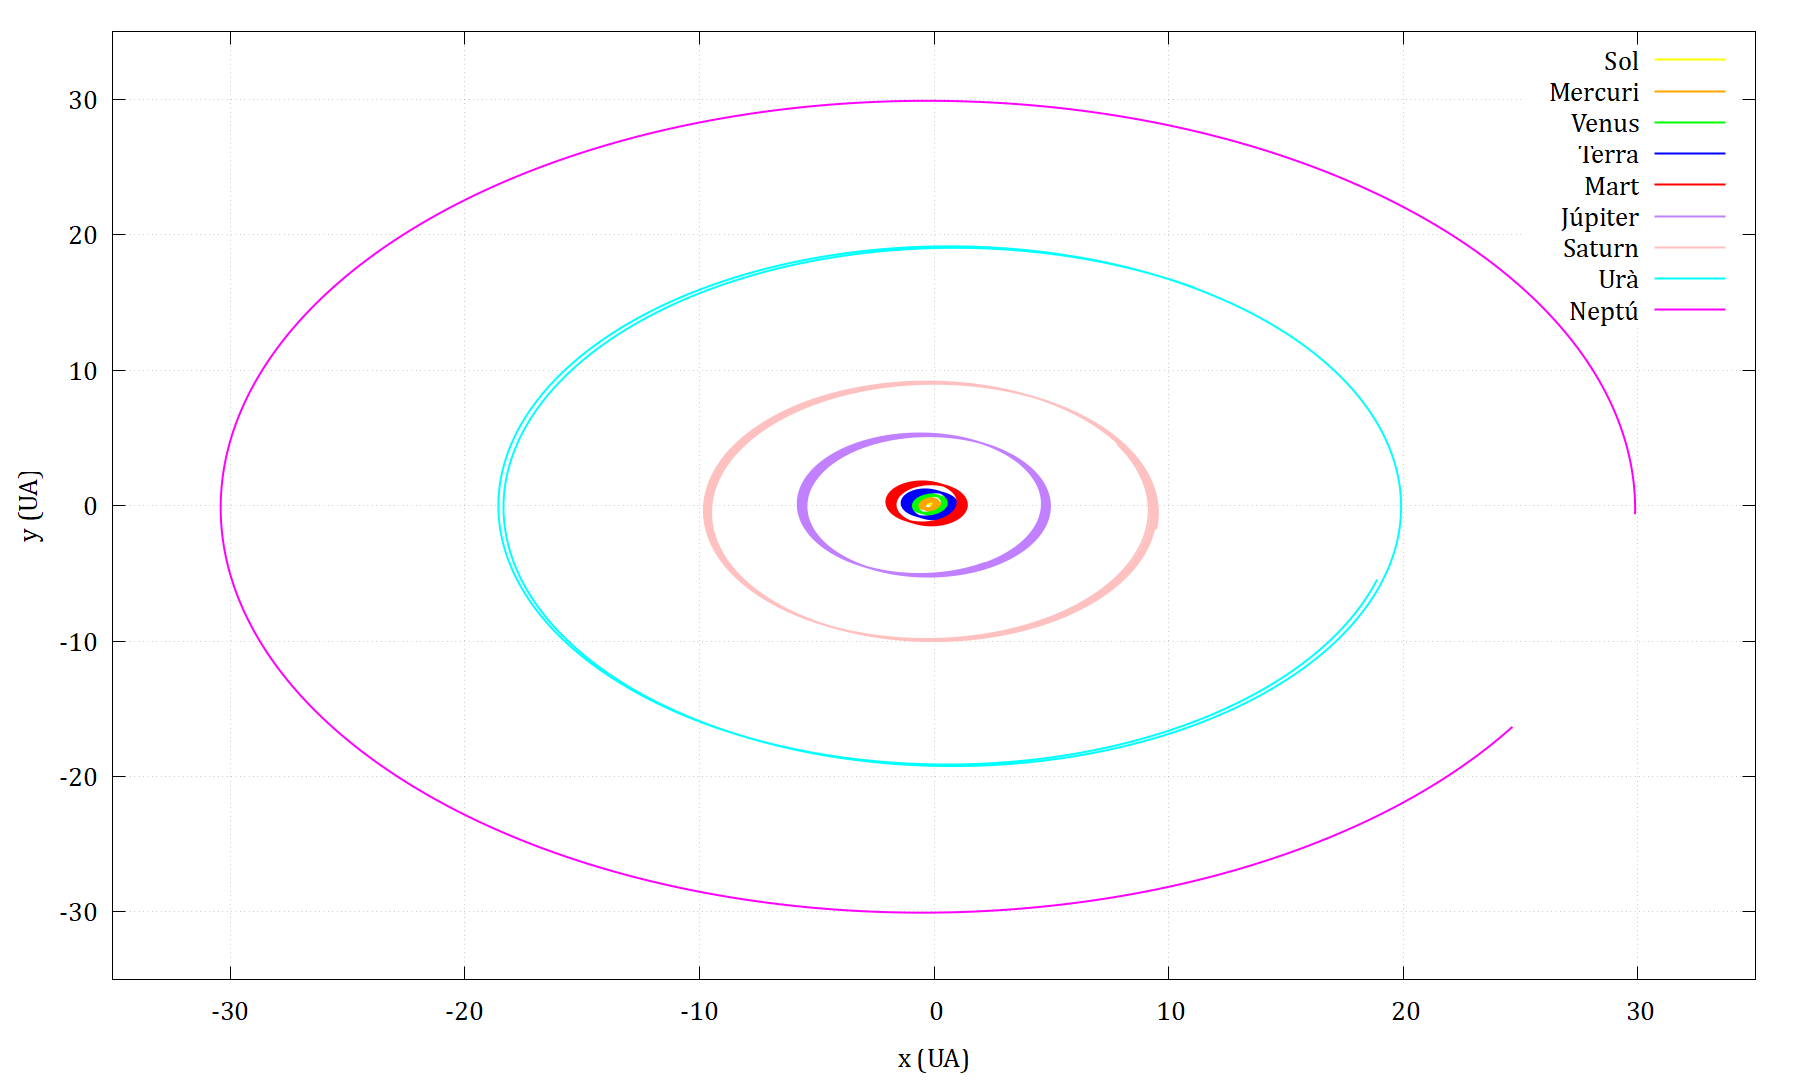
\includegraphics[width=1.0\linewidth]{../sist_solar/orbites_euler_TOTS_150_d1dia.png}
    \caption{Òrbites obtingudes amb el mètode d'Euler per a una simulació amb $dt=1$ any fins a $t_{final}=150$ anys per tots els cossos importants del Sistema Solar.}
    \label{fig:an1}
\end{figure}

Al repositori de \textit{GitHub} podreu veure una animació, a $t_{final}=15$ anys, en la que es poden veure les òrbites anteriors.

\section{Posicions i velocitats inicials dels cossos del Sistema Solar}
\label{an:c}
A continuació adjuntem les posicions i les velocitats dels diferents planetes del sistema solar (en les unitats indicades), prenent com a origen de coordenades el Sol, el dia 01/01/2025 a les 00:00 (UTC $\pm$ 00:00). Les dades han estat extretes del servei \textit{Horizon Ephemeris} de la NASA (veure \cite{ref3}).

\begin{table}[H]
\centering
\caption{Posicions i velocitats dels diferents planetes del Sistema Solar el dia 01/01/2025 a les 00:00 (UTC $\pm$ 00:00) segons l'\textit{Horizon Ephemeris} de la NASA. Es pren com a origen de coordenades la posició inicial del Sol.}
\renewcommand{\arraystretch}{1.3}
\resizebox{\textwidth}{!}{ % Redimensiona la tabla para ajustarse al ancho del texto
    \begin{tabular}{@{}lcccccc@{}}
        \specialrule{1.5pt}{0pt}{3pt} % Línea más gruesa al inicio
        \textbf{Planeta} & \textbf{\(x\) (AU)} & \textbf{\(y\) (AU)} & \textbf{\(v_x\) (AU/día)} & \textbf{\(v_y\) (AU/día)} \\ 
        \specialrule{1.2pt}{0pt}{3pt} % Segunda línea ligeramente más gruesa
        Mercuri & -0.3873030085256687 & -0.1617241946342014 & 0.005024430196457658 & -0.02474345331076241 \\ 
        Venus & 0.4534187654737982 & 0.5622160792960551 & -0.01580627428004959 & 0.01261006264179427 \\ 
        Terra & -0.1786834409731047 & 0.9669827953774551 & -0.01720473858166942 & -0.003193533189307208 \\ 
        Mart & -0.5216858665681380 & 1.525234576802456 & -0.01271183490340182 & -0.003338839586392289 \\ 
        Júpiter & 1.056033545576702 & 4.971452162023883 & -0.007476272400979211 & 0.001924466075080766 \\ 
        Saturn & 9.461067271500818 & -1.764614720843175 & 0.0007093807804551229 & 0.005475097536527790 \\ 
        Urà & 11.10363513617210 & 16.09448694134911 & -0.003273722830755306 & 0.002053528375126505 \\ 
        Neptú & 29.87992735576156 & -0.6341879950443392 & 0.00003941595250081164 & 0.003160389775728832 \\ 
        \specialrule{1.5pt}{3pt}{0pt} % Línea final más gruesa
    \end{tabular}
}
\label{tab:planets}
\end{table}

Podeu trobar un manual d'instruccions sobre com usar el servei \textit{Horizon Ephemeris} a la mateixa web de l'enllaç \cite{ref3}. 

\section{Millora del model}
\label{an:d}
Per tal d'obtenir resultats amb un nivell més elevat d'exactitud, entesa com una aproximació més propera a la realitat, es podrien implementar les següents millores pel que respecta al model considerat:
\begin{itemize}
    \item \textbf{Consideració de tots els planetes: } Tot i que el codi proporcionat està programat per a poder considerar els efectes de tots els planetes del sistema solar, a la pràctica només s'han tingut en compte els sis primers cossos. Per tant, amb una senzilla modificació del codi es podria incorporar la influència de la resta dels planetes, millorant així la precisió dels resultats.
    \item \textbf{Pla de l'eclíptica: } Com s'ha mencionat a l'informe, s'ha assumit que tots els cossos es mouen en un mateix pla, fet que no s'ajusta al sistema solar real, especialment si es vol tenir en compte la influència de Plutó \footnote{Tot i que actualment no es considera un planeta, la seva presència també genera interaccions amb la resta de cossos del sistema solar.}, el qual orbita en un pla molt diferent a l'eclíptica de la Terra i el Sol. Pel que fa als altres planetes, si bé és cert que tots orbiten en una eclíptica molt similar, hi ha uns mínims angles d'inclinació que difereixen del pla Terra-Sol.
    \item \textbf{Cossos puntuals: }Per tal de simplificar el sistema solar i poder-lo modelitzar més còmodament, els cossos, tot i tenir la massa real, es consideren puntuals. Com és evident, aquest model no es correspon a la realitat. La implementació d'aquesta millora, però, pot dificultar i donar molta més complexitat als càlculs realitzats.
\end{itemize}

\section{Millora del mètode}
\label{an:e}
Anàlogament a la secció anterior, proposarem una sèrie de millores que es podrien implementar per tal d'obtenir resultats més propers a la realitat.

El mètode numèric que hem seleccionat per aquesta pràctica ha estat el d'Euler. Aquest algorisme és de primer ordre, de manera que l'error comès és proporcional a la discretització amb què s'estigui treballant.
\begin{itemize}
    \item \textbf{Reduir la discretització: } Tot i que ja hem presentat les gràfiques d'error amb les diferents discretitzacions provades, l'interval de temps més petit és d'una hora. Així, si es continués reduint la discretització temporal, obtindríem òrbites més properes a la realitat, ja que l'error comès a cada iteració seria menor.
    \item \textbf{Altres mètodes numèrics més precisos: } Tal com s'ha treballat en l'assinatura de \textit{Mètodes Numèrics II}, hi ha mètodes més precisos que el d'Euler, com per exemple el de Runge-Kutta, el qual es fa més precís a mesura que anem augmentant-ne l'ordre.
\end{itemize}



\end{document}